\documentclass[11pt]{article}

% Increase main memory size
\usepackage{etex}
\reserveinserts{1000}
\usepackage{morewrites}
\usepackage{multicol}
\usepackage{pgfplots}
\usepackage{tikz}
\usetikzlibrary{external}
\tikzexternalize[prefix=cached_models/]

\usepackage{etex}
\reserveinserts{1000}
\usepackage{morewrites}

\listfiles

\usepackage{amsmath, amssymb, amsthm}
\usepackage{graphicx}
\usepackage{geometry}
\usepackage{array}
\usepackage{booktabs}
\usepackage{float}
\usetikzlibrary{3d}

% Page Layout
\geometry{a4paper, margin=1in}
\setlength\parindent{0pt}
\pgfplotsset{compat=1.18}

% Custom commands
\newcommand{\card}[1]{\lvert #1 \rvert}
\newcommand{\inner}[2]{\left\langle #1, #2 \right\rangle}

\title{\textbf{Vector Calculus}}
\author{}
\date{}

\begin{document}

\maketitle

\section{Euclidean space}
We define the euclidean space in $\mathbb{R}^N, N \geq 1$ using cartesian coordinates.

Any element $x \in \mathbb{R}^N, \quad x = (x_1,x_2, \dots , x_N), \quad x \in \mathbb{R}$

\subsection*{Standard basis}
\[
e_1 = (1,0, \dots ,0), \dots , e_N = (0,0, \dots ,1)
\]
\[
\text{Then, } x = \sum_{j = 1}^{N} x_j \cdot e_j
\]

In particular, $B_{\mathbb{R}^3} = \{i,j,k\}$, the canonical basis.

\subsection*{Properties}
\begin{itemize}
    \item Addition: \quad $(x_1, \dots ,x_N) + (y_1, \dots , y_N) = (x_1 + y_1, \dots , x_N + y_N)$
    \item Multiplication by a scalar $\lambda \in \mathbb{R}$: \quad $\lambda x = \lambda (x_1, \dots , x_N) = (\lambda x_1, \dots , \lambda x_N)$
    \item Associative: \quad $\lambda, \mu \in \mathbb{R}, \quad (\lambda \mu)x = \lambda(\mu x)$
    \item Additive Identity: \quad There exists a vector $\overline{0} = (0, \dots , 0)$ such that $x + \overline{0} = x$
    \item Additive Inverse: \quad $\forall x = (x_1, \dots , x_N)$, $\exists$  $\overline{x} = (-x_1, \dots , -x_N)$ such that $x + \overline{x} = \overline{0}$
    \item Distributive Property (over vector addition): 
    \begin{center}
        $\lambda \left( (x_1, \dots , x_N) + (y_1, \dots , y_N) \right) = \lambda(x_1, \dots , x_N) + \lambda(y_1, \dots , y_N)$
    \end{center} 
    \item Distributive Property (over scalar addition): 
    \begin{center}
        $(\lambda + \mu)(x_1, \dots , x_N) = \lambda(x_1, \dots , x_N) + \mu(x_1, \dots , x_N)$
    \end{center}
    \item Scalar Multiplication Identity: \quad $1 \cdot (x_1, \dots , x_N) = (x_1, \dots , x_N)$
    \item Zero Scalar Multiplication: \quad $0 \cdot (x_1, \dots , x_N) = (0, \dots , 0)$
\end{itemize}

\subsection*{Norm}

The euclidean space in $\mathbb{R}^N$ is a normal space with an associated norm function.
\[ 
\| \cdot \| : \mathbb{R}^N \rightarrow \mathbb{R}_+ \cup \{0\}
\]
\[
x = (x_1, \dots ,x_N) \rightarrow \| x \| = \sqrt{x_1^2 + \dots + x_N^2}
\]

\subsection*{Properties}
The norm satisfies the following properties:
\begin{itemize}
    \item[(a)] $\forall x \in \mathbb{R}^N$
    \begin{itemize}
        \item $\|x\| > 0 \iff x \neq 0$
        \item $\|x\| = 0 \iff x = 0$
    \end{itemize}
    \item[(b)] $\|\lambda x\| = |\lambda| \, \|x\|$
    \item[(c)] $\|x + y\| \leq \|x\| + \|y\| \quad \forall x, y \in \mathbb{R}^N$
    \begin{itemize}
        \item Triangular inequality.
    \end{itemize}
\end{itemize}


\subsection*{Remark: Distance}
We can define the distance between two elements in $\mathbb{R}^N$ as 

\[ 
dist(x,y) = \|x - y\| = \|y - x\|
\] 
\[
dist(\cdot ,\cdot) : \mathbb{R}^N \times \mathbb{R}^N \rightarrow \mathbb{R}
\]

\begin{itemize}
    \item $dist(x,y) = \|x - y\| > 0 \text{ if } x \neq y, \quad \text{and } dist(x,y) = 0 \text{ if } x = y$
    \item $dist(x,y) = \|x - y\| = \|-(y - x)\| = \|-1\| \cdot \|y - x\| = dist(y,x)$
    \item $dist(x,y) = \|x - y\| = \|x - z + z - y\| \leq \|x - z\| + \|z - y\| = dist(x,z) + dist(z,y)$ 
\end{itemize}

\subsection*{Remark}
For $\mathbb{R}$ such a distance is the absolute value, $| \cdot | : \mathbb{R} \rightarrow \mathbb{R}$

\section{Inner or scalar product}
Let $x, y$ be two vectors in $\mathbb{R}^N$, then

\[ 
x \cdot y = x_1 y_1 + \dots + x_N y_N
\]
\[
x \cdot y = \inner{x}{y} = (x,y) 
\]

\subsection{Properties}
The inner product satisfies the following properties:
\begin{itemize}
    \item $\forall x \in \mathbb{R}^N \; \langle x, x \rangle \geq 0$
    \item[] $\langle x, x \rangle = 0$ if $x = 0$
    \item Symmetric: $\langle x, y \rangle = \langle y, x \rangle$
    \item Bilinear: $\langle \lambda x + \mu y, z \rangle = \lambda \langle x, z \rangle + \mu \langle y, z \rangle$
\end{itemize}

\subsection{Cauchy-Schwartz inequality}
\[ 
|x \cdot y| \leq \|x\| \|y\|
\]

\paragraph*{Proof}
If $y = \lambda x, |\inner{x}{\lambda y}| = |\lambda| \|x\|^2 = \|x\| |\lambda| \|x\| = \|x\|\|y\|$

If $y \neq \lambda x$ (x and y are linearly independent).

Assume $z = \lambda x + y$

\[ 
0 \leq \inner{z}{z} = \inner{\lambda x + y}{\lambda x + y} = \inner{\lambda x}{\lambda x} + \inner{\lambda x}{y} + \inner{y}{\lambda x} + \inner{y}{y}
\]
\[ 
\text{Since } \|x\|^2 > 0, \quad = \lambda^2 \|x\|^2  + 2\lambda \inner{x}{y} + \|y\|^2
\]

If we represent it as a parabola in function of $\lambda$, it has no roots.

\[
\lambda = \frac{-2 \langle x, y \rangle \pm \sqrt{4 (\langle x, y \rangle)^2 - 4 \| x \|^2 \| y \|^2}}{2 \| x \|^2}
\]

So the discriminant $\leq 0$

\[
4 (\langle x, y \rangle)^2 - 4 \| x \|^2 \| y \|^2 \leq 0
\]

\[
\implies | \langle x, y \rangle | \leq \| x \| \| y \|
\]

\subsection{Theorem}
\[ 
\inner{x}{y} = \|x\| \|y\| \cos \varphi
\]

Writing $x$ and $y$ in polar coordinates:

\[ 
x_1 = \|x\| \cos \alpha, \quad x_2 = \|x\| \sin \alpha
\]
\[ 
y_1 = \|y\| \cos \beta, \quad y_2 = \|y\| \sin \beta
\]

\[
\inner{x}{y} = x_1 y_1 + x_2 y_2 = \|x\| \cos \alpha \|y\| \cos \beta + \|x\| \sin \alpha \|y\| \sin \beta
\]
\[ 
= \|x\|\|y\| (\cos \alpha \cos \beta + \sin \alpha \sin \beta)
\]
\[ 
= \|x\|\|y\| \cos(\alpha - \beta) = \|x\|\|y\| \cos \varphi
\]

\subsection*{Remark}
\[ 
\cos \varphi = \frac{\inner{x}{y}}{\|x\|\|y\|}
\]
\begin{center}
    Then $x \perp y \iff \inner{x}{y} = 0$
\end{center}

\subsection*{Examples:}
\begin{itemize}
    \item $C((a,b)) \cong \text{continuous functions in } (a,b)$
    \[
    f, g \in C((a,b)), \quad then \inner{f}{g} = \int_{a}^{b} f(t)g(t) \,dt 
    \]
    
    We can add some weights:
    \[
    \inner{f}{g} = \int_{a}^{b} w(t)f(t)g(t) \,dt 
    \]

    An example: 
    \[
    \inner{f}{g} = \int_{a}^{b} e^{-t}f(t)g(t) \,dt 
    \]
    \item We might have an orthogonal family (with infinite elements) of functions.
    \[
    \{\cos nx,\sin nx\}_{n \in \mathbb{Z}} \quad \text{in } [0,2\pi]
    \]
    \[\|\cos nx\|^2 = 
    \int_{0}^{2\pi} \cos^2 nx \,dx
    \]
    \[
    \int_{0}^{2\pi} \cos nx \sin nx \,dx = \int_{0}^{2\pi} \cos nx \cos mx \,dx = 0 \quad \text{for } n \neq m
    \]
\end{itemize}

\section{Vector Product (Only in $\mathbb{R}^3$)}

Take $x, y \in \mathbb{R}^3$

\[
x \times y = \begin{vmatrix}
i & j & k \\
x_1 & x_2 & x_3 \\
y_1 & y_2 & y_3
\end{vmatrix}
\]

\[
= \begin{vmatrix}
x_2 & x_3 \\
y_2 & y_3
\end{vmatrix} i - \begin{vmatrix}
x_1 & x_3 \\
y_1 & y_3
\end{vmatrix} j + \begin{vmatrix}
x_1 & x_2 \\
y_1 & y_2
\end{vmatrix} k
\]

Recall:

\[
\begin{vmatrix}
a & b \\
c & d
\end{vmatrix} = ad - bc
\]

\subsection{Triple product and properties}

We take the triple product

\[
a \cdot (b \times c) = (a_1, a_2, a_3) \cdot \begin{vmatrix}
b_1 & b_2 & b_3 \\
c_1 & c_2 & c_3
\end{vmatrix}
\]

\[
= a_1 \begin{vmatrix}
b_2 & b_3 \\
c_2 & c_3
\end{vmatrix} - a_2 \begin{vmatrix}
b_1 & b_3 \\
c_1 & c_3
\end{vmatrix} + a_3 \begin{vmatrix}
b_1 & b_2 \\
c_1 & c_2
\end{vmatrix}
\]

\[
= \begin{vmatrix}
a_1 & a_2 & a_3 \\
b_1 & b_2 & b_3 \\
c_1 & c_2 & c_3
\end{vmatrix}
\]

If $u \in \text{span}\{b, c\}$ then $a \cdot (b \times c) = 0$ and $a, b, c$ are coplanar if $a \cdot (b \times c) = 0$

\subsection{Geometric Interpretation}
\begin{itemize}
    \item The magnitude of $x \times y$ represents the area of the parallelogram formed by $x$ and $y$.
    \item The direction of $x \times y$ is perpendicular to the plane spanned by $x$ and $y$, following the right-hand rule.
    \item The cross product satisfies: $x \times y = - (y \times x)$.
\end{itemize}

\section{Topology of $\mathbb{R}^n$}

Definition of open spaces: we define an open ball in $\mathbb{R}^n$ centered at $x_0$ and of radius $R$.

\[
\text{Denoted by } \quad B_R(x_0) = \{ x \in \mathbb{R}^n : \text{dist}(x, x_0) < R \}
\]

This set includes all points in $\mathbb{R}^n$ whose distance from $x_0$ is less than $R$. Open sets are the building blocks of topological spaces, and they help define concepts such as convergence, continuity, and compactness.

\subsection{Open set}
A set $A \subset \mathbb{R}^n$ is open if $\forall x \in A, \quad \exists R > 0$ such that $B_R(x) \subset A$.

For example:
\[
(x,y) \in \mathbb{R}^2, \quad A = \{ (x,y) \in \mathbb{R}^2 : \sqrt{x^2 + y^2} < 3 \}
\]

\subsection{Closed set}
A set $A \subset \mathbb{R}^n$ is closed if its complement is open.
\[
A \subset \mathbb{R}^n \text{ is closed if } \mathbb{R}^n \setminus A \text{ is open.}
\]

\subsection{Boundary of a set}
The boundary of a set $A \subset \mathbb{R}^n$ denoted by $\partial A$:
\[
\partial A = \{ x \in \mathbb{R}^n : \forall R > 0, \quad B_R(x) \cap A \neq \emptyset \text{ and } B_R(x) \cap (\mathbb{R}^n \setminus A) \neq \emptyset \}
\]

Following the previous example, the boundary of $A$ is the circle of radius 3 centered at the origin:
\[
\partial A = \{ (x,y) \in \mathbb{R}^2 : \sqrt{x^2 + y^2} = 3 \}
\]

\subsection*{Remark}
A set $A \subset \mathbb{R}^n$ is closed if and only if it contains its boundary.

\subsection*{Example:}
\[
D = \{(x,y) \in \mathbb{R}^2 : \sqrt{x^2 + y^2} < 1 \text{ and } x > 0\}
\]

\[
D^C = \{(x,y) \in \mathbb{R}^2 : \sqrt{x^2 + y^2} \geq 1 \text{ or } x \leq 0\}
\]

\[
\partial D = \{(x,y) \in \mathbb{R}^2 : \sqrt{x^2 + y^2} = 1 \text{ and } x > 0\}
\]

$D$ is open, $D^C$ is closed, and $\partial D$ is the semicircle of radius 1 centered at the origin.

\subsection*{Example:}
\[
S = \{x = 1 \text{ and } 1 < y \leq 2\}
\]

\[
S^C = \{x \neq 1 \text{ or } y \leq 1 \text{ or } y > 2\}
\]

\[
\partial S = \{x = 1 \text{ and } y = 1 \text{ or } y = 2\}
\]

$S$ is neither open nor closed, as $S^C$, and $\partial S$ is the line segment from $(1,1)$ to $(1,2)$.

\subsection{Compact set}   
A set $A \subset \mathbb{R}^n$ is compact if and only if it is closed and bounded.

\subsection*{Example:}
\[
A = \{(x,y) \in \mathbb{R}^2 : x^2 + y^2 = 4\}
\]

$A = \partial A$ so $A$ is closed. $A$ is also bounded, as all points in $A$ are contained within the circle of radius 2 centered at the origin.

$\implies A$ is compact.

\subsection*{Example: (Exercise 11a)}
\[
A = xy-\text{plane in } \mathbb{R}^3 = \{(x,y,0) \in \mathbb{R}^3\}
\]

This set is closed, and $B_R(x, R) \cap A = \emptyset$ and $B_R(x, R) \cap (\mathbb{R}^3 \setminus A) = \emptyset$.

Therefore, $A$ is will not be compact.

\subsection*{Example: (Exercise 11b)}
\[
A = \{(x,y) \in \mathbb{R}^2 : xy \ne 0\}
\]

For any point $(x,y) \in A$, we can find an open ball $B_R(x, R) \subset B$ that does not intersect the $x$ or $y$ axes.
\[
R = \min\{x, y\}
\]

\subsection{Ball in $\mathbb{R}^n$}
For a ball at any part of radius $r$ in $\mathbb{R}^n$:
\[
(x_1 - a_1)^2 + \dots + (x_n - a_n)^2 < r^2
\]
\[
\text{dist}(x - a) = \|x - a\| = r
\]

\subsection*{Example: (Exercise 1a)}
Sphere centered at (0,1,-1) with $r = 4$
\[
(x-0)^2 + (y-1)^2 + (z+1)^2 = 16
\]

Intersection with the $x,y,z$-planes:
\[
\text{If } z = -1, \quad x^2 + (y-1)^2 = 16
\]
\[
\text{If } y = 1, \quad x^2 + (z+1)^2 = 16
\]
\[
\text{If } x = 0, \quad (y-1)^2 + (z+1)^2 = 16
\]

\subsection*{Example: (Exercise 1b)}
Sphere going through the origin and centered at $(1,2,3)$:
\[
(x-1)^2 + (y-2)^2 + (z-3)^2 = r^2
\]
\[
\text{dist}(0, (1,2,3)) = \sqrt{1^2 + 2^2 + 3^2} = \sqrt{14}
\]

So the sphere is $(x-1)^2 + (y-2)^2 + (z-3)^2 = 14$

\subsection*{Example: (Exercise 1c)}
Find center and radius of the sphere:
\[
x^2 + y^2 + z^2 + 2x + 8y - 4z = 28
\]
\[
(x+1)^2 + (y+4)^2 + (z-2)^2 = 49
\]

So the center is $(-1,-4,2)$ and the radius is $7$.

\subsection*{Example: (Exercise 3)}
Check if the vectors are orthogonal:
\[
a = (-5,3,7), \quad b = (6,-8,2)
\]
\[
a \cdot b = -30 - 24 + 14 = -40 != 0
\]
So $a$ and $b$ are not orthogonal.

\subsection*{Example: (Exercise 4a)}
Let P be a point not on the line L that passes through the points Q and R. Show that the
distance d from the point P to the line L is:
\[
d = \frac{\|a \times b\|}{\|a\|}
\]

\[
\text{Let } a = R - Q, \quad b =  P - Q
\]
\[
\text{Then } d = \frac{\|a \times b\|}{\|a\|}
\]
\[
\text{Area of parallelogram} = \|a \times b\| = \|a\| \cdot d
\]

\subsection*{Example: (Exercise 4b)}
Use the formula in part (a) to find the distance from the point $P(1, 1, 1)$ to the line through $Q(0, 6, 8)$ and $R(-1, 4, 7)$.

\[
\mathbf{a} = \overrightarrow{QR} = R - Q = (-1 - 0, 4 - 6, 7 - 8) = (-1, -2, -1)
\]
\[
\mathbf{b} = \overrightarrow{QP} = P - Q = (1 - 0, 1 - 6, 1 - 8) = (1, -5, -7)
\]

\[
\mathbf{a} \times \mathbf{b} =
\begin{vmatrix}
\mathbf{i} & \mathbf{j} & \mathbf{k} \\
-1 & -2 & -1 \\
1 & -5 & -7
\end{vmatrix}
\quad
= \mathbf{i} \begin{vmatrix} -2 & -1 \\ -5 & -7 \end{vmatrix}
- \mathbf{j} \begin{vmatrix} -1 & -1 \\ 1 & -7 \end{vmatrix}
+ \mathbf{k} \begin{vmatrix} -1 & -2 \\ 1 & -5 \end{vmatrix}
\]

\[
\mathbf{a} \times \mathbf{b} = (9, -8, 7)
\]

\[
\|\mathbf{a} \times \mathbf{b}\| = \sqrt{9^2 + (-8)^2 + 7^2}
= \sqrt{81 + 64 + 49} = \sqrt{194}
\]
\[
\|\mathbf{a}\| = \sqrt{(-1)^2 + (-2)^2 + (-1)^2} = \sqrt{1 + 4 + 1} = \sqrt{6}
\]

\[
d = \frac{\|\mathbf{a} \times \mathbf{b}\|}{\|\mathbf{a}\|} = \frac{\sqrt{194}}{\sqrt{6}}
= \sqrt{\frac{194}{6}} = \sqrt{\frac{97}{3}}
\]

\subsection*{Example: (Exercise 5)}
Calculate the volume of the parallelepiped with edges adjacent to $\overrightarrow{PQ}$, $\overrightarrow{PR}$, and $\overrightarrow{PS}$,
where
\[
P(1, 1, 1), \quad Q(2, 0, 3), \quad R(4, 1, 7), \quad S(3, -1, -2).
\]

The volume of the parallelepiped can be calculated using the scalar triple product of the vectors $\overrightarrow{PQ}$, $\overrightarrow{PR}$, and $\overrightarrow{PS}$.

\[
\overrightarrow{PQ} = Q - P = (2 - 1, 0 - 1, 3 - 1) = (1, -1, 2)
\]
\[
\overrightarrow{PR} = R - P = (4 - 1, 1 - 1, 7 - 1) = (3, 0, 6)
\]
\[
\overrightarrow{PS} = S - P = (3 - 1, -1 - 1, -2 - 1) = (2, -2, -3)
\]

\[
\overrightarrow{PR} \times \overrightarrow{PS} = \begin{vmatrix}
\mathbf{i} & \mathbf{j} & \mathbf{k} \\
3 & 0 & 6 \\
2 & -2 & -3
\end{vmatrix}
= \mathbf{i}(0 \cdot (-3) - 6 \cdot (-2)) - \mathbf{j}(3 \cdot (-3) - 6 \cdot 2) + \mathbf{k}(3 \cdot (-2) - 0 \cdot 2)
\]
\[
= \mathbf{i}(0 + 12) - \mathbf{j}(-9 - 12) + \mathbf{k}(-6 - 0)
\]
\[
= 12\mathbf{i} + 21\mathbf{j} - 6\mathbf{k}
\]
\[
= (12, 21, -6)
\]

\[
\overrightarrow{PQ} \cdot (\overrightarrow{PR} \times \overrightarrow{PS}) = (1, -1, 2) \cdot (12, 21, -6)
\]
\[
= 1 \cdot 12 + (-1) \cdot 21 + 2 \cdot (-6)
\]
\[
= 12 - 21 - 12
\]
\[
= -21
\]

The volume of the parallelepiped is the absolute value of this scalar triple product:
\[
\text{Volume} = | -21 | = 21
\]

\subsection*{Example: (Exercise 6)}
Use the scalar product to check if the following vectors are coplanar:
$a = 2i + 3j + k, b = i - j$ and $c = 7i + 3j + 2k$.

The vectors are coplanar if the scalar triple product of the vectors is zero.

\[
\mathbf{b} \times \mathbf{c} =
\begin{vmatrix}
\mathbf{i} & \mathbf{j} & \mathbf{k} \\
1 & -1 & 0 \\
7 & 3 & 2
\end{vmatrix}
\quad 
= (-2, -2, 10)
\]

\[
\mathbf{a} \cdot (-2, -2, 10) = (2 \times -2) + (3 \times -2) + (1 \times 10)
\]
\[
= -4 - 6 + 10 = 0
\]

Since the scalar triple product is zero, the vectors are coplanar.

\section{Functions of several variables}
A function $f : A \rightarrow B$ is a correspondence between two sets $A$ and $B$ such that each element in $A$ is associated with exactly one element in $B$.

\subsection*{Example:}
\[
f(x,y) = x^2 + y^2 \quad \text{, where }
\]
\[
f : \mathbb{R}^2 \rightarrow \mathbb{R}
\]
\[
(x,y) \rightarrow f(x,y) = x^2 + y^2
\]

The formula for that function:
\[
z = x^2 + y^2
\]

The graph results in a paraboloid (surface).

\subsection{Domain for a function $f$}
The domain is the set of points where the function is well defined.

\subsection{Image of a function $f$}
The image is the set of points in $B$ that are associated with points in $A$.

\subsection*{Example: (Exercise 8)}
\begin{itemize}
    \item The function \[ x^2 + 2z^2 = 1 \] is a cylinder with an elipse section.
    \item The function \[ x^2 - y^2 + z^2 = 1 \]
    \begin{itemize}
        \item If $y = k$, then $x^2 + z^2 = 1 + k^2$ is a circle.
        \item If $z = 0$, then $x^2 - y^2 = 1$ is a hyperbola.
        \item If $x = 0$, then $z^2 - y^2 = 1$ is a hyperbola.
    \end{itemize}
\end{itemize}

\subsection{Types of functions}
\begin{itemize}
    \item Scalar functions: $f : \mathbb{R}^n \rightarrow \mathbb{R}$, \quad $f(x_1, \dots , x_n) \in \mathbb{R}$.
    \item Vector functions: $f : \mathbb{R}^n \rightarrow \mathbb{R}^m$, \quad $f(x_1, \dots , x_n) \in \mathbb{R}^m$. \\
                         If $f : \mathbb{R}^n \rightarrow \mathbb{R}^n$, then $f$ is a vector field.
\end{itemize}

\subsection*{Example:}
Paramatric equations for a line in $\mathbb{R}^3$:
\[
\begin{cases}
x = x_0 + at \\
y = y_0 + bt \\
z = z_0 + ct
\end{cases}
\]

\subsection{Level curves}
The level curves of a function $f : \mathbb{R}^N \rightarrow \mathbb{R}$ are the curves in the domain of $f$ where $f(x,y) = k$ for some constant $k$.

\[
(x_1, \dots , x_N) \rightarrow f(x_1, \dots , x_N) \in \mathbb{R}
\]
\[
f(x,y) = c, \quad c \in \mathbb{R}
\]

The graph of a scalar function $f : \mathbb{R}^2 \rightarrow \mathbb{R}$ is a surface in $\mathbb{R}^3$.

\subsection*{Example:}
\[
f(x,y) = x^2 + y^2
\]
\[
x^2 + y^2 = c, \quad c \in \mathbb{R}
\]

The level curves are circles centered at the origin.
They can be seen as the projection of the surface onto the $xy$-plane (from above).

\subsection{Remark}
In $\mathbb{R}^3$, the level curves of a function $f : \mathbb{R}^3 \rightarrow \mathbb{R}$ are the curves in the domain of $f$ where $f(x,y,z) = c$ for some constant $c \in \mathbb{R}$.

They allow us to visualize a 3D graph of a function in 2D.

If the level curves are very close to each other, then the function is steep.

Two level curves never touch.

\subsection*{Example:}
Find the level curves of the function $f(x,y) = xy$.

\[
xy = c, \quad c = 1, -1, 2.
\]

\begin{center}
    \tikzsetnextfilename{graph1}
    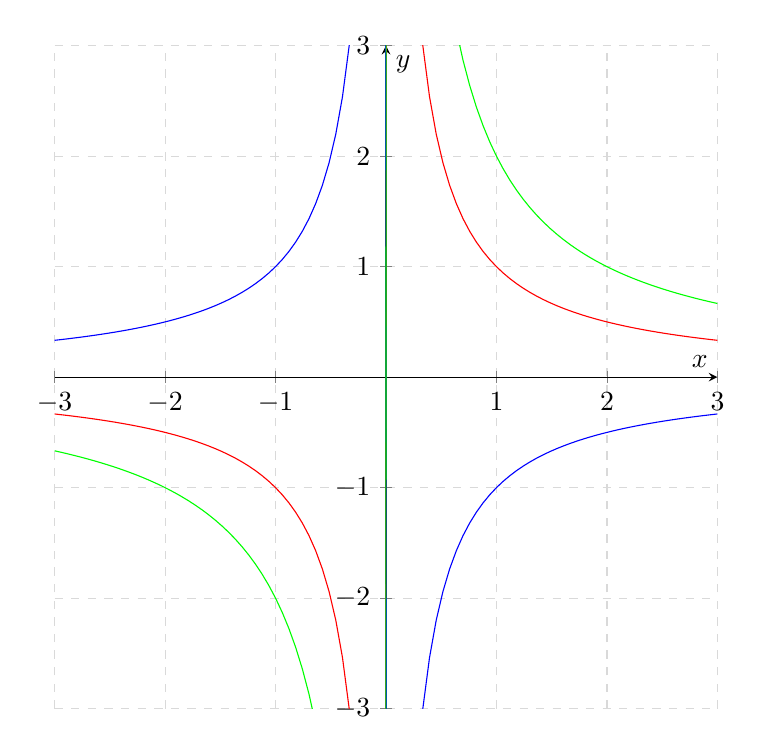
\begin{tikzpicture}
        \begin{axis}[
            axis lines = middle,
            xlabel = $x$,
            ylabel = $y$,
            xmin = -3, xmax = 3,
            ymin = -3, ymax = 3,
            width=10cm,
            height=10cm,
            grid = major,
            grid style = {dashed, gray!30},
            samples=100
        ]
        \addplot[
            domain=-3:3,
            samples=100,
            color=red
        ]
        {1/x};
        \addplot[
            domain=-3:3,
            samples=100,
            color=blue
        ]
        {-1/x};
        \addplot[
            domain=-3:3,
            samples=100,
            color=green
        ]
        {2/x};
        \end{axis}
    \end{tikzpicture}
\end{center}

The level curves are a family of hyperbolas.

\subsection*{Example:}
Find the level curves of the function $f(x,y) = log(x - y)$.

\[
log(x - y) = c, \quad c = 1, -1, 0.
\]

\begin{center}
    \tikzsetnextfilename{graph2}
    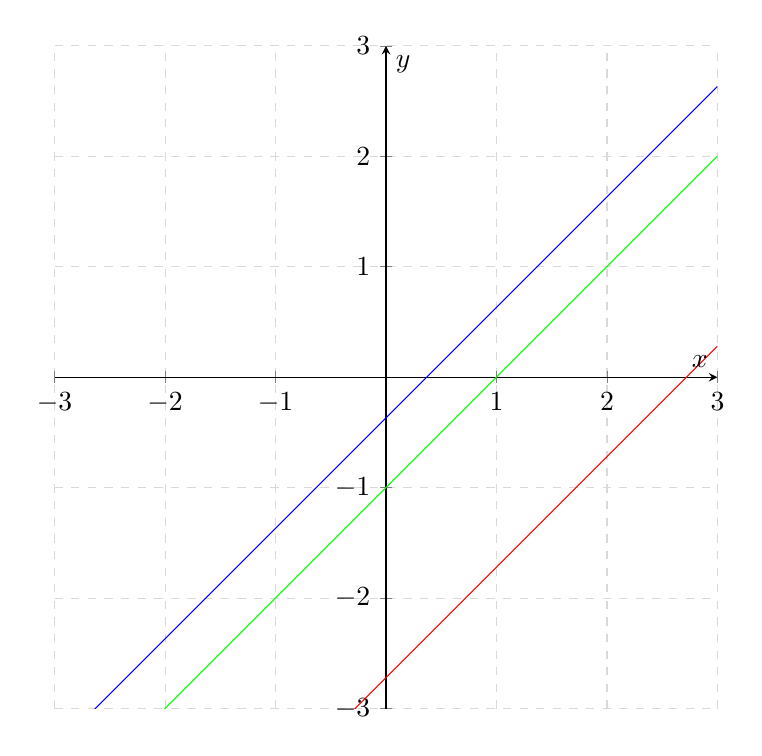
\begin{tikzpicture}
        \begin{axis}[
            axis lines = middle,
            xlabel = $x$,
            ylabel = $y$,
            xmin = -3, xmax = 3,
            ymin = -3, ymax = 3,
            width=10cm,
            height=10cm,
            grid = major,
            grid style = {dashed, gray!30},
            samples=100
        ]
        \addplot[
            domain=-3:3,
            samples=100,
            color=red
        ]
        {x - exp(1)};
        \addplot[
            domain=-3:3,
            samples=100,
            color=blue
        ]
        {x - 1/exp(1)};
        \addplot[
            domain=-3:3,
            samples=100,
            color=green
        ]
        {x - 1};
        \end{axis}
    \end{tikzpicture}
\end{center}

The level curves are a family of straight lines.

\subsection*{Example:}
Find the level curves of the functions
\[ f(x,y,z) = x^2 + y^2 + z^2 \quad \text{ and } \quad g(x,y,z) = \frac{x^2}{25} + \frac{y^2}{16} + \frac{z^2}{9} \]

The level curves for $f$ are spheres centered at the origin.

The level curves for $g$ are ellipsoids centered at the origin.

\begin{center}
    \tikzsetnextfilename{model1}
    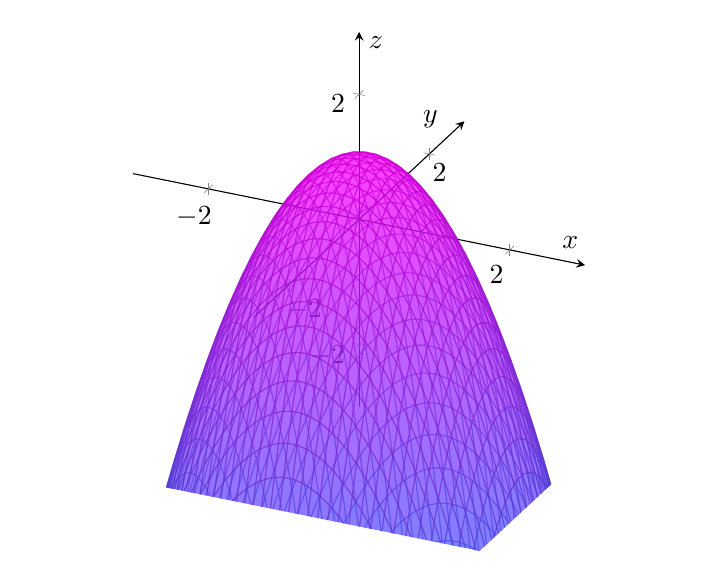
\begin{tikzpicture}
        \begin{axis}[
            axis lines = middle,
            xlabel = $x$,
            ylabel = $y$,
            zlabel = $z$,
            xmin = -3, xmax = 3,
            ymin = -3, ymax = 3,
            zmin = -3, zmax = 3,
            width=10cm,
            height=10cm,
            grid = major,
            grid style = {dashed, gray!30},
            samples=50,
            colormap/cool,
        ]
        \addplot3[
            domain=-3:3,
            samples=50,
            surf,
            opacity=0.5
        ]
        {sqrt{1 - x^2 - y^2}};
        \end{axis}
    \end{tikzpicture}
\end{center}

\begin{center}
    \tikzsetnextfilename{model2}
    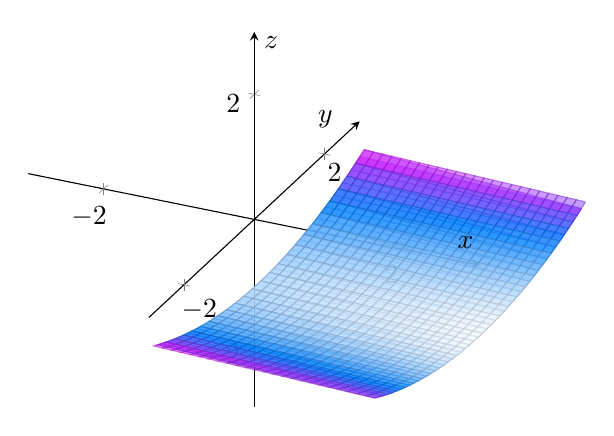
\begin{tikzpicture}
        \begin{axis}[
            axis lines = middle,
            xlabel = $x$,
            ylabel = $y$,
            zlabel = $z$,
            xmin = -3, xmax = 3,
            ymin = -3, ymax = 3,
            zmin = -3, zmax = 3,
            width=10cm,
            height=10cm,
            grid = major,
            grid style = {dashed, gray!30},
            samples=50,
            colormap/cool
        ]
        \addplot3[
            domain=-3:3,
            samples=50,
            surf,
            opacity=0.5
        ]
        {- sqrt{x^2/25 + y^2/16 - 1}};
        \end{axis}
    \end{tikzpicture}
\end{center}

\subsection{Graph of a function}
\[
\{(x, f(x)), x \in Dom(f)\}, \quad \text{where } f = 9y^2 + 4z^2 = x^2 + 36
\]

Intersection with the $x,y,z$-planes:

\[
\text{If } z = 0, \quad 9y^2 - x^2 = 36 \rightarrow \text{Hyperbola}
\]
\[
\text{If } y = 0, \quad 4z^2 - x^2 = 36 \rightarrow \text{Hyperbola}
\]
\[
\text{If } x = 0, \quad 9y^2 + 4z^2 = 36 \rightarrow \text{Ellipse}
\]

\subsection*{Example:}
Plot the function $f = x^2 + 4y^2 = z^2$.

\[
\text{If } z = 0, \quad x^2 + 4y^2 = 0 \rightarrow x = 0, y = 0
\]
\[
\text{If } y = 0, \quad x^2 = z^2 \rightarrow x = z, x = -z
\]
\[
\text{If } x = 0, \quad 4y^2 = z^2 \rightarrow y = z/2, y = -z/2
\]
\[
\text{If } z = k, \quad x^2 + 4y^2 = k^2 \rightarrow \text{Ellipses}
\]

\begin{center}
    \tikzsetnextfilename{model3}
    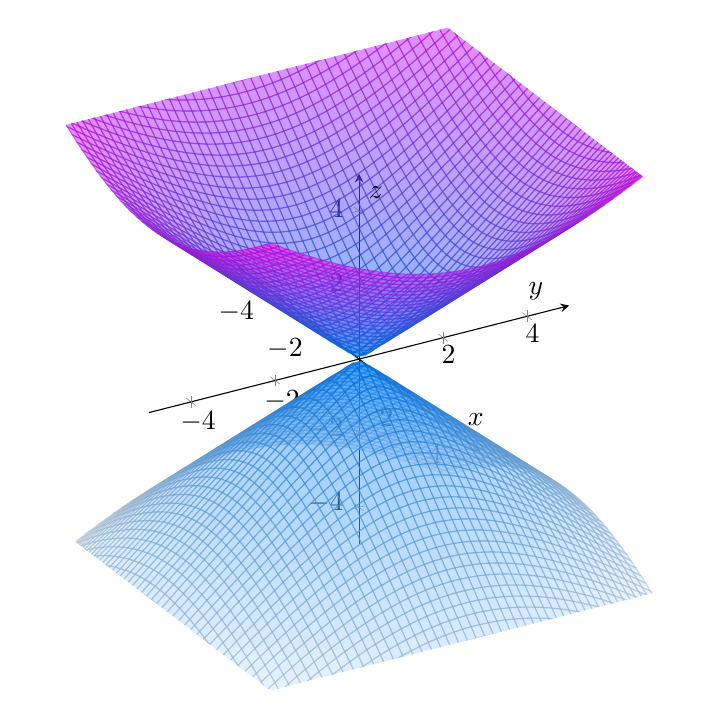
\begin{tikzpicture}
        \begin{axis}[
            axis lines = middle,
            xlabel = $x$,
            ylabel = $y$,
            zlabel = $z$,
            xmin = -5, xmax = 5,
            ymin = -5, ymax = 5,
            zmin = -5, zmax = 5,
            width=10cm,
            height=10cm,
            grid = major,
            grid style = {dashed, gray!30},
            samples=50,
            colormap/cool,
            view={60}{30}
        ]
        \addplot3[
            domain=-5:5,
            samples=50,
            surf,
            opacity=0.5
        ]
        {sqrt(x^2 + y^2)};
        \addplot3[
            domain=-5:5,
            samples=50,
            surf,
            opacity=0.5
        ]
        {-sqrt(x^2 + y^2)};
        \end{axis}
    \end{tikzpicture}
\end{center}

The graph is a cone.

\subsection*{Problem 8}
\[
x^2 + y^2 + 9z^2 = 1 \rightarrow \text{Ellipsoid}
\]
\[
x^2 - y^2 + z^2 = 1 \rightarrow \text{Hyperboloid of one sheet}
\]
\[
y = 2x^2 + z^2 \rightarrow \text{Paraboloid}
\]

\begin{center}
    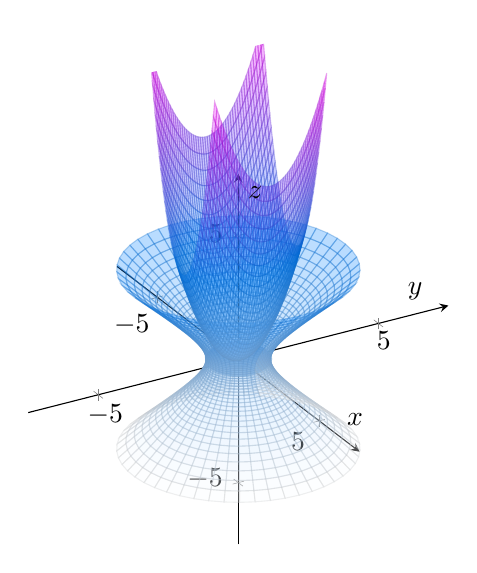
\begin{tikzpicture}
        \begin{axis}[axis lines = middle, xlabel = $x$, ylabel = $y$, zlabel = $z$, xmin = -7.5, xmax = 7.5, ymin = -7.5, ymax = 7.5, zmin = -7.5, zmax = 7.5, width=10cm, height=10cm, grid = major, grid style = {dashed, gray!30}, samples=50, samples y=50, colormap/cool, view={60}{30}]
        % Ellipsoid
        \addplot3[domain=0:pi, y domain=0:2*pi, surf, opacity=0.3]
        ({sin(deg(x))*cos(deg(y))}, {sin(deg(x))*sin(deg(y))}, {cos(deg(x))/3});
        % Hyperboloid of one sheet
        \addplot3[domain=-2:2, y domain=0:2*pi, surf, opacity=0.3]
        ({cosh(x)*cos(deg(y))}, {cosh(x)*sin(deg(y))}, {sinh(x)});
        % Paraboloid
        \addplot3[domain=-2:2, y domain=-2:2, surf, opacity=0.3]
        ({x}, {y}, {2*x^2 + y^2});
        \end{axis}
    \end{tikzpicture}
\end{center}

\subsection*{Example:}

\[
- x^2 + y^2 - z^2 = 1 \rightarrow \text{Hyperboloid}
\]
\[
\text{If } z = 0, \quad - x^2 + y^2 = 1 \rightarrow \text{Hyperbola}
\]
\[
\text{If } y = 0, \quad - x^2 - z^2 = 1 \rightarrow \text{No solution}
\]
\[
\text{If } x = 0, \quad y^2 - z^2 = 1 \rightarrow \text{Hyperbola}
\]

\begin{center}
    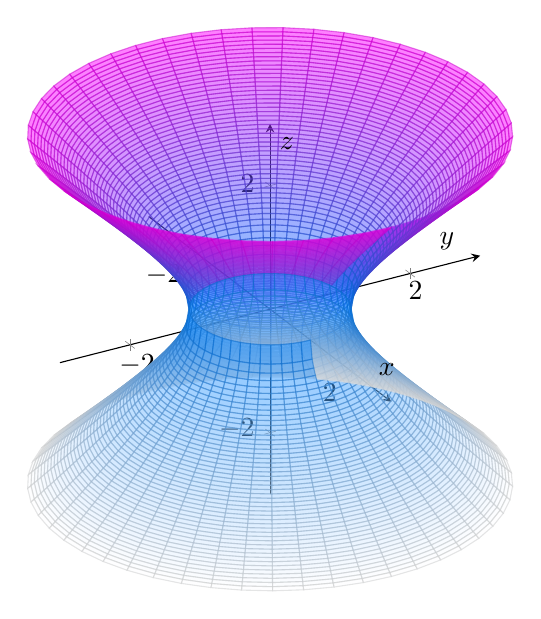
\begin{tikzpicture}
        \begin{axis}[
            axis lines = middle,
            xlabel = {$x$},
            ylabel = {$y$},
            zlabel = {$z$},
            xmin = -3, xmax = 3,
            ymin = -3, ymax = 3,
            zmin = -3, zmax = 3,
            width=10cm,
            height=10cm,
            grid = major,
            grid style = {dashed, gray!30},
            samples=50,
            samples y=50,
            colormap/cool,
            view={60}{30}
        ]
        % Upper sheet
        \addplot3[
            domain=1:3, % r starts from 1
            y domain=0:360,
            surf,
            opacity=0.5
        ]
        ({x*cos(y)}, {x*sin(y)}, {sqrt(x^2 - 1)});

        % Lower sheet
        \addplot3[
            domain=1:3,
            y domain=0:360,
            surf,
            opacity=0.5
        ]
        ({x*cos(y)}, {x*sin(y)}, {-sqrt(x^2 - 1)});
        \end{axis}
    \end{tikzpicture}
\end{center}

\subsection*{Example:}

\[
z = x^2 - y^2 \rightarrow \text{Paraboloid}
\]

\[
\text{If } z = 0, \quad x^2 - y^2 = 0 \rightarrow \text{Hyperbola}
\]
\[
\text{If } z = k, \quad x^2 = y^2 + k \rightarrow \text{Hyperbola}
\]
\[
\text{If } y = 0, \quad z = x^2 \rightarrow \text{Parabola}
\]
\[
\text{If } x = 0, \quad z = -y^2 \rightarrow \text{Parabola}
\]

\begin{center}
    \tikzsetnextfilename{model8}
    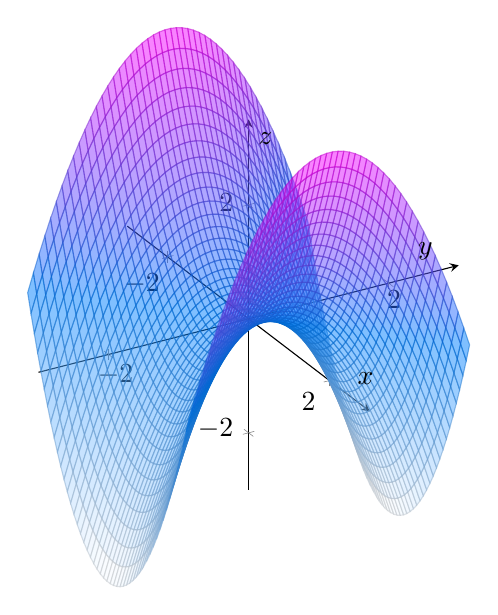
\begin{tikzpicture}
        \begin{axis}[
            axis lines = middle,
            xlabel = $x$,
            ylabel = $y$,
            zlabel = $z$,
            xmin = -3, xmax = 3,
            ymin = -3, ymax = 3,
            zmin = -3, zmax = 3.5,
            width=10cm,
            height=10cm,
            grid = major,
            grid style = {dashed, gray!30},
            samples=50,
            colormap/cool,
            view={60}{30}
        ]
        \addplot3[
            domain=-2:2,
            y domain=-2:2,
            surf,
            opacity=0.5
        ]
        {x^2 - y^2};
        \end{axis}
    \end{tikzpicture}
\end{center}

\subsection*{Example:}
Plot the function $x^2 + y^2 = 1$.

\begin{center}
    \tikzsetnextfilename{model10}
    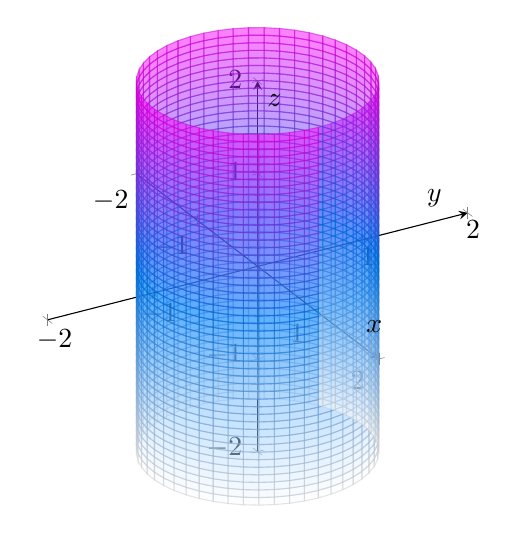
\begin{tikzpicture}
        \begin{axis}[
            axis lines = middle,
            xlabel = $x$,
            ylabel = $y$,
            zlabel = $z$,
            xmin = -2, xmax = 2,
            ymin = -2, ymax = 2,
            zmin = -2, zmax = 2,
            width=10cm,
            height=10cm,
            grid = major,
            grid style = {dashed, gray!30},
            samples=50,
            colormap/cool,
            view={60}{30}
        ]
        \addplot3[
            domain=-2:2,
            y domain=0:2*pi,
            surf,
            opacity=0.5
        ]
        ({cos(deg(y))}, {sin(deg(y))}, x);
        \end{axis}
    \end{tikzpicture}
\end{center}

\section{Cartesian coordinates in $\mathbb{R}^N$}
In $\mathbb{R}^2$, the Cartesian coordinates are $(x,y)$.

In $\mathbb{R}^3$, the Cartesian coordinates are $(x,y,z)$.

\subsection{Polar coordinates in $\mathbb{R}^2$}
\[
x = r \cos(\theta), \quad y = r \sin(\theta), \quad r \geq 0, \quad 0 \leq \theta < 2\pi
\]

Inverse transformation:
\[
r = \sqrt{x^2 + y^2}, \quad \theta = \arctan\left(\frac{y}{x}\right)
\]

\paragraph{Lemma}
Let $A = (0, \inf) \times (0, 2\pi)$. 

The function $g : A \rightarrow \mathbb{R}^2$ defined by $g(r, \theta) = (r \cos(\theta), r \sin(\theta))$ is a bijection, \\
continuous in a ball $B(0, \alpha)$ such that $\{g(r, \theta), 0 < r < \alpha, 0 -leq \theta < 2\pi\}$ is a subset of $B(0, \alpha)$.

To see if the function is one-to-one, assume that $g(r_1, \theta_1) = f(r_2, \theta_2)$ for $r_1, r_2 \geq 0$ and $0 \leq \theta_1, \theta_2 < 2\pi$.

Then $r_1 \cos(\theta_1) = r_2 \cos(\theta_2)$ and $r_1 \sin(\theta_1) = r_2 \sin(\theta_2)$. This implies that $r_1 = r_2$, since $r_1 \geq 0$ and $0 \leq \theta_1, \theta_2 < 2\pi$.

As a consequence $\theta_1 = \theta_2$ so that $g$ is one-to-one.

Now taking $(x,y) \in B(0, \alpha)$, and $r = \sqrt{x^2 + y^2} > 0$.

Then, the part $(\frac{x}{2}, \frac{y}{2})$ is in $B(0, 1)$.

Therefore, there exists $\theta \in \left[0, 2\pi\right)$ such that $\cos(\theta) = \frac{x}{r}$ and $\sin(\theta) = \frac{y}{r}$.

Which implies that $x = r \cos(\theta)$ and $y = r \sin(\theta)$. So $g$ is onto.

\subsection{Cylindrical coordinates in $\mathbb{R}^3$}
\[
x = r \cos(\theta), \quad y = r \sin(\theta), \quad z = z
\]

\begin{center}
    \tikzsetnextfilename{model11}
    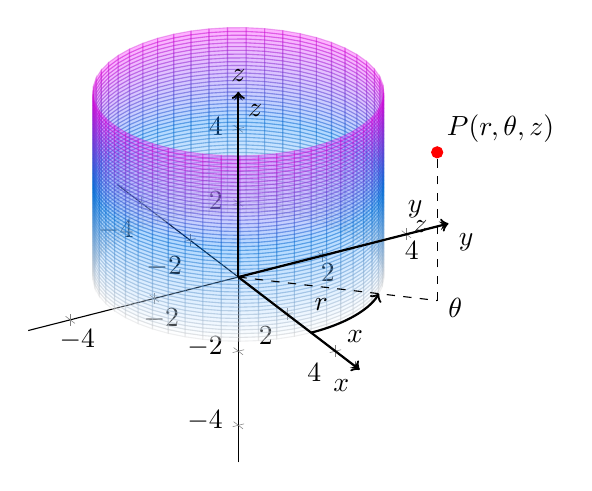
\begin{tikzpicture}
        \begin{axis}[
            axis lines = middle,
            xlabel = $x$,
            ylabel = $y$,
            zlabel = $z$,
            xmin = -5, xmax = 5,
            ymin = -5, ymax = 5,
            zmin = -5, zmax = 5,
            width=10cm,
            height=10cm,
            view={60}{30},
            grid = major,
            grid style = {dashed, gray!30},
            samples=50,
            colormap/cool,
        ]
        \addplot3[domain=0:2*pi, y domain=0:5, surf, opacity=0.3]
        ({3*cos(deg(x))}, {3*sin(deg(x))}, y);
        
        \draw[thick,->] (axis cs:0,0,0) -- (axis cs:5,0,0) node[anchor=north east] {$x$};
        \draw[thick,->] (axis cs:0,0,0) -- (axis cs:0,5,0) node[anchor=north west] {$y$};
        \draw[thick,->] (axis cs:0,0,0) -- (axis cs:0,0,5) node[anchor=south] {$z$};
        
        \addplot3[mark=*, color=red] coordinates {(3, 3, 4)};
        \node at (axis cs:3, 3, 4) [anchor=south west] {$P(r, \theta, z)$};
        
        \draw[dashed] (axis cs:0,0,0) -- (axis cs:3, 3, 0) node[midway, anchor=north east] {$r$};
        
        \draw[thick,->] (axis cs:3,0,0) arc[start angle=0, end angle=45, radius=3] node[midway, anchor=south] {$\theta$};
        
        \draw[dashed] (axis cs:3, 3, 0) -- (axis cs:3, 3, 4) node[midway, anchor=east] {$z$};
        
        \end{axis}
    \end{tikzpicture}
\end{center}

\subsection*{Example:}
Transform into cartesian coordinates:
\[
(3, \frac{\pi}{2}, 1) = (3 \cos(\frac{\pi}{2}), 3 \sin(\frac{\pi}{2}), 1) = (0, 3, 1)
\]

\subsection*{Example:}
Transform into cartesian coordinates:
\[
(4, - \frac{\pi}{3}, 5) = (4 \cos(-\frac{\pi}{3}), 4 \sin(-\frac{\pi}{3}), 5) = (2, -2\sqrt{3}, 5)
\]

\subsection{Spherical coordinates in $\mathbb{R}^3$}
\[
x = \rho \sin(\phi) \cos(\theta), \quad y = \rho \sin(\phi) \sin(\theta), \quad z = \rho \cos(\phi), \quad \rho \geq 0, \quad 0 \leq \phi \leq \pi, \quad 0 \leq \theta < 2\pi
\]

$\rho$ is the distance from the origin, $\phi$ is the angle from the $z$-axis, and $\theta$ is the angle from the $x$-axis.

\begin{center}
    \tikzsetnextfilename{model12}
    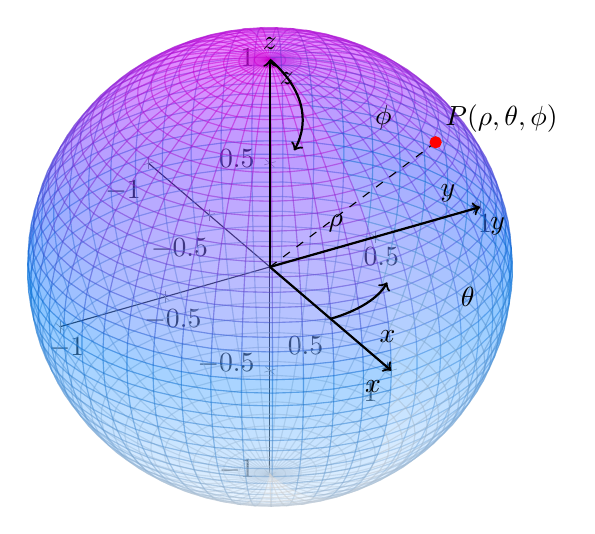
\begin{tikzpicture}
        \begin{axis}[
            axis lines = middle,
            xlabel = $x$,
            ylabel = $y$,
            zlabel = $z$,
            xmin = -1, xmax = 1,
            ymin = -1, ymax = 1,
            zmin = -1, zmax = 1,
            width=10cm,
            height=11cm,
            view={60}{30},
            grid = major,
            grid style = {dashed, gray!30},
            samples=50,
            colormap/cool,
        ]
        \addplot3[
            domain=0:pi,
            y domain=0:2*pi,
            surf,
            opacity=0.3,
        ]
        ({sin(deg(x))*cos(deg(y))}, {sin(deg(x))*sin(deg(y))}, {cos(deg(x))});
        
        \draw[thick,->] (axis cs:0,0,0) -- (axis cs:1,0,0) node[anchor=north east] {$x$};
        \draw[thick,->] (axis cs:0,0,0) -- (axis cs:0,1,0) node[anchor=north west] {$y$};
        \draw[thick,->] (axis cs:0,0,0) -- (axis cs:0,0,1) node[anchor=south] {$z$};
        
        \addplot3[mark=*, color=red] coordinates {(0.5, 0.5, 0.707)};
        \node at (axis cs:0.5, 0.5, 0.707) [anchor=south west] {$P(\rho, \theta, \phi)$};
        
        \draw[dashed] (axis cs:0,0,0) -- (axis cs:0.5, 0.5, 0.707) node[midway, anchor=north east] {$\rho$};
        
        \draw[thick,->] (axis cs:0.5,0,0) arc[start angle=0, end angle=45, radius=0.5] node[midway, anchor=south] {$\theta$};
        
        \draw[thick,->] (axis cs:0,0,1) arc[start angle=90, end angle=45, radius=1] node[midway, anchor=east] {$\phi$};
        
        \end{axis}
    \end{tikzpicture}
\end{center}

\subsection*{Example: (Problem 6)}
Transform into spherical coordinates:
\[
(1,0,0) = (1 \sin(\phi) \cos(\theta), 1 \sin(\phi) \sin(\theta), 1 \cos(\phi)) = (0,0,1)
\]

\[
(2,\frac{\pi}{3},\frac{\pi}{4}) = (2 \sin(\frac{\pi}{4}) \cos(\frac{\pi}{3}), 2 \sin(\frac{\pi}{4}) \sin(\frac{\pi}{3}), 2 \cos(\frac{\pi}{4})) = (\sqrt{3}, 1, \sqrt{2})
\]

\subsection{Parametric equation of a line in $\mathbb{R}^3$}
Having two points $P_1(x_1, y_1, z_1)$ and $P_2(x_2, y_2, z_2)$, the parametric equation of the line passing through $P_1$ and $P_2$ is:
\[
\begin{cases}
x = x_1 + t(x_2 - x_1) \\
y = y_1 + t(y_2 - y_1) \\
z = z_1 + t(z_2 - z_1)
\end{cases}
\]

\subsection*{Example: (Problem 14)}
Find the parametric equation of the line passing through $P(1,0,1)$ and $Q(2,3, 1)$.

\[
\begin{cases}
x = 1 + t(2 - 1) = 1 + t \\
y = 0 + t(3 - 0) = 3t \\
z = 1 + t(1 - 1) = 1
\end{cases}
\]

\subsection{Parametric equation of a plane in $\mathbb{R}^3$}
For a plane in parametric form:
\[
\begin{cases}
x = x_0 + a_1 t + a_2 s \\
y = y_0 + b_1 t + b_2 s \\
z = z_0 + c_1 t + c_2 s
\end{cases}
\]

\paragraph{Remark}
A line in $\mathbb{R}^3$ is a manifold of dimension 1. \\
A plane in $\mathbb{R}^3$ is a manifold of dimension 2.

\subsection*{Example: (Problem 9)}
$\text{Write } x^2 + y^2 + z^2 = 4 \text{ (Sphere)} \text{ in parametric form}$.

\[
\begin{cases}
    x = \lambda \\
    y = \mu \\
    z = \sqrt{4 - \lambda^2 - \mu^2}
\end{cases}
\quad \text{where } \lambda^2 + \mu^2 \leq 4
\]

Using spherical coordinates:
\[
\begin{cases}
    x = \rho \sin(\phi) \cos(\theta) \\
    y = \rho \sin(\phi) \sin(\theta) \\
    z = \rho \cos(\phi)
\end{cases}
\quad \text{where } 0 \leq \phi \leq \pi, \quad 0 \leq \theta < 2\pi, \quad \rho = 2
\]
\[
\rho^2\cos^2(\theta)\sin^2(\phi) + \rho^2\sin^2(\theta)\sin^2(\phi) + \rho^2\cos^2(\phi) = 4
\]
\[
\rho^2\sin^2(\phi)(\cos^2(\theta) + \sin^2(\theta)) + \rho^2\cos^2(\phi) = 4
\]
\[
\rho^2\sin^2(\phi) + \rho^2\cos^2(\phi) = 4
\]
\[
\rho^2 = 4 \rightarrow \rho = 2
\]

\subsection*{Example: (Problem 11)}
A solid above the cone $z = \sqrt{x^2 + y^2}$ and below the sphere $x^2 + y^2 + z^2 = z$.

\[
\text{Becase the solid is inside the cone, we have } z \geq \sqrt{x^2 + y^2}
\]
\[
\text{Because the solid is below the sphere, we have } x^2 + y^2 + z^2 \leq z
\]

\[
\begin{cases}
    x = \rho \sin(\phi) \cos(\theta) \\
    y = \rho \sin(\phi) \sin(\theta) \\
    z = \rho \cos(\phi)
\end{cases}
\quad \text{where } 0 \leq \phi \leq \pi, \quad 0 \leq \theta < 2\pi
\]

\[
\sqrt{\rho^2\cos^2(\theta)\sin^2(\phi) + \rho^2\sin^2(\theta)\sin^2(\phi)} \leq \rho\cos(\phi)
\]
\[
\rho\sin(\phi) \leq \rho\cos(\phi) \rightarrow \tan(\phi) \leq 1 \rightarrow \phi \leq \frac{\pi}{4}
\]

\[
\rho^2\sin^2(\phi)(\cos^2(\theta) + \sin^2(\theta)) + \rho^2\cos^2(\phi) \leq \rho\cos(\phi)
\]
\[
\rho^2\sin^2(\phi) + \rho^2\cos^2(\phi) \leq \rho\cos(\phi)
\]
\[  
\rho^2 \leq \rho\cos(\phi) \rightarrow \rho \leq \cos(\phi)
\]

\begin{center}
    \tikzsetnextfilename{solid}
    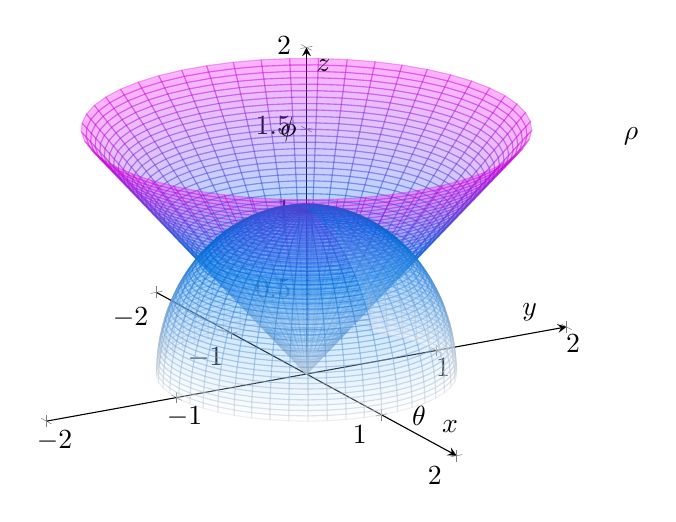
\begin{tikzpicture}
        \begin{axis}[
            axis lines = middle,
            xlabel = $x$,
            ylabel = $y$,
            zlabel = $z$,
            xmin = -2, xmax = 2,
            ymin = -2, ymax = 2,
            zmin = 0, zmax = 2,
            width=12cm,
            height=9cm,
            view={60}{30},
            grid = major,
            grid style = {dashed, gray!30},
            samples=50,
            colormap/cool,
        ]
        % Cone
        \addplot3[domain=0:2*pi, y domain=0:1.5, surf, opacity=0.3]
        ({y*cos(deg(x))}, {y*sin(deg(x))}, y);
        
        % Sphere
        \addplot3[domain=0:pi/2, y domain=0:2*pi, surf, opacity=0.3]
        ({cos(deg(x))*cos(deg(y))}, {cos(deg(x))*sin(deg(y))}, {sin(deg(x))});
        
        % Labels
        \node at (axis cs:1.5, 1.5, 1.5) [anchor=south west] {$\rho$};
        \node at (axis cs:1.5, 0, 0) [anchor=south] {$\theta$};
        \node at (axis cs:0, 0, 1.5) [anchor=east] {$\phi$};
        
        \end{axis}
    \end{tikzpicture}
\end{center}

Solid in cartesian coordinates:
\[
\begin{cases}
    z \geq \sqrt{x^2 + y^2} \\
    x^2 + y^2 + z^2 \leq z
\end{cases}
\]

In spherical coordinates:
\[
\begin{cases}
    \rho \leq \cos(\phi) \\
    \phi \leq \frac{\pi}{4} \\ 
    \theta \in [0, 2\pi)
\end{cases}
\]

\subsection{Intersection of two bodies}
The intersection of two bodies gives (in general) a curve.

\subsection*{Example: (Problem 12)}
Parametrize the intersection (a curve $\gamma(t) = (\gamma_1(t), \gamma_2(t), \gamma_3(t))$) of the two bodies:
\[
\begin{cases}
    \text{Cylinder: } x^2 + y^2 = 4 \\
    \text{Surface: } z = xy
\end{cases}
\]

\[
\begin{cases}
    x = 2\cos(t) = \gamma_1(t) \\
    y = 2\sin(t) = \gamma_2(t) \\
    z = 2\cos(t)\sin(t) = \gamma_3(t)
\end{cases}
\text{ where } t \in [0, 2\pi)
\]

\begin{center}
    \tikzsetnextfilename{cylinder_surface}
    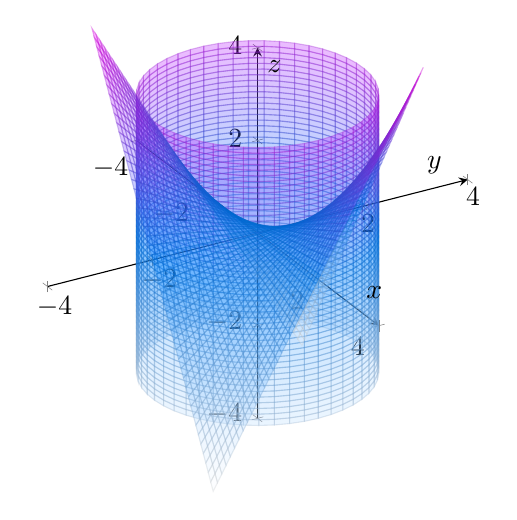
\begin{tikzpicture}
        \begin{axis}[
            axis lines = middle,
            xlabel = $x$,
            ylabel = $y$,
            zlabel = $z$,
            xmin = -4, xmax = 4,
            ymin = -4, ymax = 4,
            zmin = -4, zmax = 4,
            width=10cm,
            height=10cm,
            view={60}{30},
            grid = major,
            grid style = {dashed, gray!30},
            samples=50,
            colormap/cool,
        ]
        % Cylinder
        \addplot3[domain=0:2*pi, y domain=-3:3, surf, opacity=0.3]
        ({2*cos(deg(x))}, {2*sin(deg(x))}, y);
        
        % Surface
        \addplot3[domain=-2:2, y domain=-2:2, surf, opacity=0.3]
        (x, y, {x*y});
        \end{axis}
    \end{tikzpicture}
\end{center}

\[
\begin{cases}
    \text{Paraboloid: } z = 4x^2 + y \\
    \text{Cylinder: } y = x^2
\end{cases}
\implies 
\begin{cases}
    x = t \\
    y = t^2 \\
    z = 4t^2 + t^4
\end{cases}
\]

\begin{center}
    \tikzsetnextfilename{paraboloid_cylinder}
    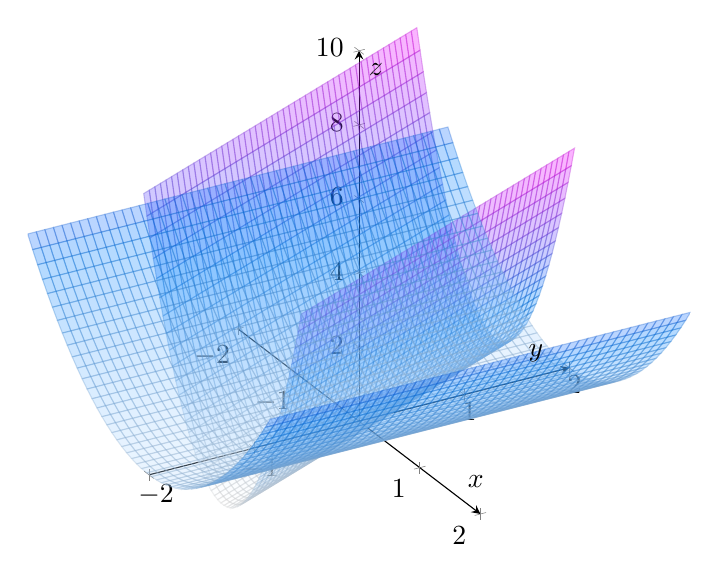
\begin{tikzpicture}
        \begin{axis}[
            axis lines = middle,
            xlabel = $x$,
            ylabel = $y$,
            zlabel = $z$,
            xmin = -2, xmax = 2,
            ymin = -2, ymax = 2,
            zmin = 0, zmax = 10,
            width=10cm,
            height=10cm,
            view={60}{30},
            grid = major,
            grid style = {dashed, gray!30},
            samples=50,
            colormap/cool,
        ]
        % Paraboloid
        \addplot3[
            domain=-1.3:1.3,
            y domain=-1.3:1.3,
            samples=50,
            surf,
            opacity=0.3
        ]
        {4*x^2 + y};
        
        % Cylinder
        \addplot3[
            domain=-2:2,
            y domain=-2:2,
            samples=50,
            surf,
            opacity=0.3
        ]
        {x^2};        
        \end{axis}
    \end{tikzpicture}
\end{center}

\section{Limit of functions}
Assume a scalar $f : \mathbb{R}^N \rightarrow \mathbb{R}$.
We say that the limit of $f(x)$ as $x$ approaches $x_0$ is $L$ and we denote it by:
\[
\lim_{x \to x_0} f(x) = L \quad \in \mathbb{R}, \quad x, x_0 \in \mathbb{R}^N
\]

\subsection{Definition of the limit}
We say that $\lim_{x \to x_0} f(x) = L$ if for every $\epsilon > 0$ there exists $\delta > 0$ such that:
\[
\forall x \in \mathbb{R}^N, \quad 0 < ||x - x_0|| < \delta \implies |f(x) - L| < \epsilon
\]

\paragraph{Theorem}
If the limit of $f(x)$ as $x$ approaches $x_0$ exists, then the limit is unique.

\paragraph{Proof}
Argue by contradiction. Assume that there are two limits $L_1$ and $L_2$ such that $L_1 \neq L_2$.
\vskip 0.5cm
Actually, we can say that:
\[
B(L_1, r_1) \cap B(L_2, r_2) = \emptyset
\]

Where $B(L_1, r_1)$ is the ball of radius $r_1$ centered at $L_1$ and $B(L_2, r_2)$ is the ball of radius $r_2$ centered at $L_2$.
\[
\lim_{x \to x_0} f(x) = L_1, \quad \text{for any } \epsilon_1 > 0, \quad \exists \delta_1 > 0 \text{ such that } |f(x) - L_1| < \epsilon_1 \text{ for } 0 < ||x - x_0|| < \delta_1
\]
\[
\lim_{x \to x_0} f(x) = L_2, \quad \text{for any } \epsilon_2 > 0, \quad \exists \delta_2 > 0 \text{ such that } |f(x) - L_2| < \epsilon_2 \text{ for } 0 < ||x - x_0|| < \delta_2
\]

Indeed, 
\[
\begin{cases}
    |f(x) - L_1| < r_1 = \epsilon_1 \\
    |f(x) - L_2| < r_2 = \epsilon_2
\end{cases}
\implies \text{However, taking } \delta = \min(\delta_1, \delta_2) \text{ so that } ||x - x_0|| < \delta
\]

\[
\text{such that } 
\begin{cases}
    |f(x) - L_1| < \min(r_1 , r_2) \\
    |f(x) - L_2| < \min(r_1 , r_2) 
\end{cases}    
\implies L_1 = L_2, \text{ which is a contradiction}
\]

\subsection{Computing limits}
Using the definition of the limit, we can compute the limit of a function $f(x)$ as $x$ approaches $x_0$. To do so we must choose the value of $L$ towards the function is going. The process is as follows:
\[
\text{For example in } \mathbb{R}^2, \quad 
\begin{cases}
    f : \mathbb{R}^2 \rightarrow \mathbb{R} \\
    (x,y) \rightarrow f(x,y)
\end{cases}
\]

Then:
\[
0 < \sqrt{(x - x_0)^2 + (y - y_0)^2} < \delta \implies |f(x,y) - L| < \epsilon
\]

Hence, we must find $\delta \cong \delta(\epsilon)$.

\subsection*{Example:}
Prove that 
\[
\lim_{(x,y) \to (0,0)} \sqrt{x^2 + y^2} \sin\left(\frac{1}{x^2 + y^2}\right) = 0
\]

\[
\text{Let } \epsilon > 0, \quad \text{we must find } \delta > 0 \text{ such taht } \left|\sqrt{x^2 + y^2} \sin\left(\frac{1}{x^2 + y^2}\right)\right| < \epsilon
\]

\[
\text{Since } \left|\sin\left(\frac{1}{x^2 + y^2}\right)\right| \leq 1 \text{ and } \sqrt{x^2 + y^2} \geq 0
\]

\[
\text{We have } \left|\sqrt{x^2 + y^2} \sin\left(\frac{1}{x^2 + y^2}\right)\right| \leq \sqrt{x^2 + y^2} < \epsilon
\]

\[
\text{Therefore, we can choose } \delta = \epsilon
\]

\subsection*{Example:}
Prove that
\[
\lim_{(x,y) \to (a,b)} y = b
\]

\[
\text{Let } \epsilon > 0, \quad \text{we must find } \delta > 0 \text{ such that } ||f(x) - b|| = |y - b| < \epsilon
\]
\[
\text{when } ||(x,y) - (a,b)|| = \sqrt{(x-a)^2 + (y-b)^2} < \delta
\]

\[
\text{We start from } |y - b| \leq \sqrt{(x-a)^2 + (y-b)^2} < \delta
\]
\[
\text{Therefore, we can choose } \delta = \epsilon
\]

\subsection{Iterative limits}
In 2D, 
\[
\lim_{x \to a} \left(\lim_{y \to b} f(x,y)\right) = \lim_{y \to b} \left(\lim_{x \to a} f(x,y)\right)
\]

However, this technique only gives us negative answers (non-existence of the limit). Since we are just following one direction.

\subsection{Approach following families of functions}
They might be straight lines, parabolas, etc. around the point of approach.

\subsection*{Example:}
Compute the limit:
\[
\lim_{(x,y) \to (0,0)} \frac{x}{\sqrt{x^2 + y^2}}
\]

Let y = $\lambda x, \quad \lambda \in \mathbb{R}$. Then
\[
\lim_{(x,y) \to (0,0)} \frac{x}{\sqrt{x^2 + y^2}} = \lim_{x \to 0} \frac{x}{\sqrt{x^2 + \lambda^2 x^2}} = \lim_{x \to 0} \frac{x}{|x|\sqrt{1 + \lambda^2}} = \frac{1}{\sqrt{1 + \lambda^2}}
\]

This limit depends on $\lambda$. Therefore, the limit does not exist.

\subsection*{Example:}
Compute the limit:
\[
\lim_{(x,y) \to (0,0)} \frac{x^3}{x^2 + y^2}
\]

Let $y = \lambda x, \quad \lambda \in \mathbb{R}$. Then
\[
\lim_{(x,y) \to (0,0)} \frac{x^3}{x^2 + y^2} = \lim_{x \to 0} \frac{x^3}{x^2 + \lambda^2 x^2} = \lim_{x \to 0} \frac{x}{1 + \lambda^2} = 0
\]

Following the family of functions $y = \lambda x$, the limit is 0. However, we cannot confirm that the value of the limit is 0 or that the limit exists using this method.
\vskip 0.5cm
This method is necessary but not sufficient. It is a good way to check if the limit does not exist.

\subsection*{Problem 1a}
Taking $y = \lambda x$ and knowing that $\sin x \approx x$ for $x \approx 0$:
\[
\lim_{(x,y) \to (0,0)} \frac{x^2 + \sin^2 y}{2x^2 + y^2} = \lim_{x \to 0} \frac{x^2 + \sin^2(\lambda x)}{2x^2 + \lambda^2x^2} = \lim_{x \to 0} \frac{x^2 + \lambda^2 x^2}{2x^2 + \lambda^2x^2} = \frac{1 + \lambda^2}{2 + \lambda^2}
\]

This limit depends on $\lambda$. Therefore, the limit does not exist.

\subsection*{Problem 1d}
Taking $y = \lambda x$:
\[
\lim_{(x,y) \to (0,0)} \frac{xy}{\sqrt{x^2 + y^2}} = \lim_{x \to 0} \frac{x\lambda x}{\sqrt{x^2 + \lambda^2 x^2}} = \lim_{x \to 0} \frac{\lambda x^2}{\sqrt{x^2(1 + \lambda^2)}} = \lim_{x \to 0} \frac{\lambda x}{\sqrt{1 + \lambda^2}} = 0
\]

This limit does not depend on $\lambda$. Therefore, the limit exists and is 0.

Using polar coordinates:
\[
\lim_{(x,y) \to (0,0)} \frac{xy}{\sqrt{x^2 + y^2}} = \lim_{r \to 0} \frac{r^2 \cos(\theta) \sin(\theta)}{r} = \lim_{r \to 0} r \cos(\theta) \sin(\theta) = 0
\]

\subsection{Polar coordinates}
In $\mathbb{R}^2$, the polar coordinates are $(r, \theta)$.
\[
x = r \cos(\theta), \quad y = r \sin(\theta), \quad r \geq 0, \quad 0 \leq \theta < 2\pi
\]

\paragraph{Theorem}
Let us consider two functions $f$ and $g$ such that
\[
\lim_{x \to x_0} f(x) = 0, \quad \text{and } g \text{ is bounded for } ||x - x_0|| < \delta
\]

Then
\[
\lim_{x \to x_0} f(x)g(x) = 0
\]

\subsection*{Problem 1e}
Taking $y = \lambda x$:
\[
\lim_{(x,y) \to (0,0)} \frac{x^2 ye^y}{x^4 + 4y^2} = \lim_{x \to 0} \frac{x^2 \lambda x e^{\lambda x}}{x^4 + 4\lambda^2 x^2} = \lim_{x \to 0} \frac{\lambda x^3 e^{\lambda x}}{x^2(x^2 + 4\lambda^2)} = \lim_{x \to 0} \frac{\lambda x e^{\lambda x}}{x^2 + 4\lambda^2} = 0
\]

Now taking $y = x^2$:
\[
\lim_{(x,y) \to (0,0)} \frac{x^2 ye^y}{x^4 + 4y^2} = \lim_{x \to 0} \frac{x^2 x^2 e^{x^2}}{x^4 + 4x^4} = \lim_{x \to 0} \frac{x^4 e^{x^2}}{5x^4} = \lim_{x \to 0} \frac{e^{x^2}}{5} = \frac{1}{5}
\]

This limit depends on the direction of approach. Therefore, the limit does not exist.

\subsection*{Problem 1f}
Applying generalized spherical coordinates:

\[
\begin{cases}
    x = r \sin(\phi) \cos(\theta) \\
    y = \frac{1}{2} r \sin(\phi) \sin(\theta) \\
    z = \frac{1}{3} r \cos(\phi)
\end{cases}
\]

\[
\lim_{(x,y,z) \to (0,0,0)} \frac{yz}{x^2 + 4y^2 + 9z^2} = \lim_{r \to 0} \frac{\frac{1}{2} r \sin(\phi) \sin(\theta) \frac{1}{3} r \cos(\phi)}{r^2} = \lim_{r \to 0} \frac{1}{6} \sin(\phi) \cos(\phi) \sin(\theta)
\]

This limit depends on $\phi$ and $\theta$. Therefore, the limit does not exist.

\section{Continuity of functions}
A function $f : \mathbb{R}^N \rightarrow \mathbb{R}$ is continuous at $x_0 \in \mathbb{R}^N$ if:
\begin{enumerate}
    \item $f(x_0)$ is defined.
    \item $\lim_{x \to x_0} f(x)$ exists.
    \item $\lim_{x \to x_0} f(x) = f(x_0)$
\end{enumerate}

\paragraph{Theorem}
Consider $A$ a subset in $\mathbb{R}^N$ and $f : A \rightarrow \mathbb{R}^M$ a vector function. 
\[
F(x) = (f_1(x), f_2(x), \ldots, f_M(x))
\]

If $f_1, f_2, \ldots, f_M$ are continuous at $x_0 \in A$, then $F$ is continuous at $x_0$.

\paragraph{Theorem}
Assume that $f$ and $g$ are continuous at $x_0 \in \mathbb{R}^N$ and $f(x_0)$ respectively. Then, the composition $g \circ f$ is continuous at $x_0$.
\[
\text{For example: } f(x) = x^2y \sin(x + y), \quad f : \mathbb{R}^2 \rightarrow \mathbb{R}
\]

Since $f$ is a composite function and $x^2, y, \sin(x + y)$ are continuous, then $f$ is continuous.

\subsection*{Problem 2a}
Prove the continuity:
\[
f(x,y) = 
\begin{cases}
    \dfrac{x^2y^3}{2x^2 + y^2} & \text{if } (x,y) \neq (0,0) \\
    1 & \text{if } (x,y) = (0,0)
\end{cases}
\]

If $(x,y) \neq (0,0)$, then $f(x,y)$ is a composition of continuous functions. So that 
\[
\text{for any } (x_0,y_0) \neq (0,0), \quad \lim_{(x,y) \to (0,0)} f(x,y) = f(x_0,y_0) = \dfrac{x_0^2y_0^3}{2x_0^2 + y_0^2}
\]

At $(0,0)$, the function is well defined: $f(0,0) = 1$, so we must check that the limit exists.
\[
\lim_{(x,y) \to (0,0)} f(x,y) = \lim_{(x,y) \to (0,0)} \frac{x^2y^3}{2x^2 + y^2} = 
\]

Using polar coordinates:
\[
\begin{cases}
    x = \dfrac{1}{\sqrt{2}}r \cos(\theta) \\
    y = r \sin(\theta)
\end{cases}
\]

\[
= \lim_{r \to 0} \dfrac{\frac{1}{2} r^3 \cos^2(\theta) \sin^3(\theta)}{r^2} = \lim_{r \to 0} \frac{1}{2} r \cos^2(\theta) \sin^3(\theta) = 0
\]

The limit exists and is equal to 0. However, $f(0,0) = 1 \neq 0$. Therefore, the function is not continuous at $(0,0)$.

\subsection*{Problem 3}
\[
f(x,y) = 
\begin{cases}
    0 & \text{if } y \leq 0 \text{ or } y \geq x^4 \\
    1 & \text{if } 0 < y < x^4
\end{cases}
\]

a) $lim_{(x,y) \to (0,0)} f(x,y) = 0$ along any path going through $y = mx^\alpha$. \quad $0 < \alpha < 4$

\begin{center}
    \tikzsetnextfilename{plot_fxy_3d}
    \begin{tikzpicture}
        \begin{axis}[
            axis lines = middle,
            xlabel = {$x$},
            ylabel = {$y$},
            zlabel = {$f(x,y)$},
            xmin = -2, xmax = 2,
            ymin = -2, ymax = 2,
            zmin = -0.5, zmax = 1.5,
            width=10cm,
            height=10cm,
            view={120}{30},
            samples=200,
            colormap/cool,
        ]
        \addplot3[
            domain=-2:2,
            y domain=-2:2,
            surf,
            opacity=0.5
        ]
        {y <= 0 ? 0 : (y >= x^4 ? 0 : 1)};
        \end{axis}
    \end{tikzpicture}
\end{center}

Let $\alpha = 1$: $y = mx$. Then
\[
\lim_{(x,y) \to (0,0)} f(x,y) = \lim_{x \to 0} f(x,mx) = \lim_{x \to 0} f(x,mx) = 0
\]

In this case, the limit exists and is equal to 0.
\vskip 0.5cm
b) Despite (a), prove that the function is not continuous.

Take any point $(a,0), \quad a \in \mathbb{R}$. Then:
\[
\lim_{(x,y) \to (a,0)} f(x,y) = 
\begin{cases}
    0 & \text{if } y \to 0^- \\
    1 & \text{if } y \to 0^+
\end{cases}
\]

The limit depends on the direction of approach. Therefore, the function is not continuous.
\vskip 0.5cm
c) $f$ discontinuous on two entire curves:
$\begin{cases}
    y = x^4 \\
    y = 0
\end{cases}$

Take any point $(a,a^4)$ on $y = x^4, \quad a \in \mathbb{R}$. Then:
\[
lim_{(x,y) \to (a,a^4)} f(x,y) = 
\]
\[
||(x,y) - (a,a^4)|| < \delta \implies
\begin{cases}
    0 < |f(x,y)| = 1 < \epsilon & \text{if } y < x^4 \\
    0 < |f(x,y)| = 0 < \epsilon & \text{if } y > x^4
\end{cases}
\]

The limit depends on the direction of approach. Therefore, the function is not continuous.

\subsection*{Example:}
Consider the function:
\[
f(x,y) =
\begin{cases}
    \dfrac{x^3y}{x^6 + y^2} & \text{if } (x,y) \neq (0,0) \\
    0 & \text{if } (x,y) = (0,0)
\end{cases}
\]

Let $y = \lambda x, \quad \lambda \in \mathbb{R}$. Then
\[
a) \lim_{(x,y) \to (0,0)} \frac{x^3y}{x^6 + y^2} = \lim_{x \to 0} \frac{x^3 \lambda x}{x^6 + \lambda^2 x^2} = \lim_{x \to 0} \frac{\lambda x^2}{x^4 + \lambda^2} = 0
\]

Now taking $y = x^3$:
\[
b) \lim_{(x,y) \to (0,0)} \frac{x^3y}{x^6 + y^2} = \lim_{x \to 0} \frac{x^3 x^3}{x^6 + x^6} = \lim_{x \to 0} \frac{x^6}{2x^6} = \frac{1}{2}
\]

Therefore the function is not continuous at $(0,0)$, since the limit depends on the direction of approach.

\section{Differentiability of functions}
In 1D when we consider a function $f : \mathbb{R} \rightarrow \mathbb{R}$, the derivative of $f$ at $a \in \mathbb{R}$ describes the ratio of the change of the function $f$ at $x = a$ and is denoted by:
\[
f'(a) = \lim_{t \to 0} \frac{f(a + t) - f(a)}{t} = \frac{df(a)}{dt}
\]

Geometrically, the derivative of a function at a point is the slope of the tangent line to the curve at that point. And this tangent line is defined as:
\[
y = f(a) + f'(a)(x - a)
\]

\begin{center}
    \tikzsetnextfilename{tangent_line}
    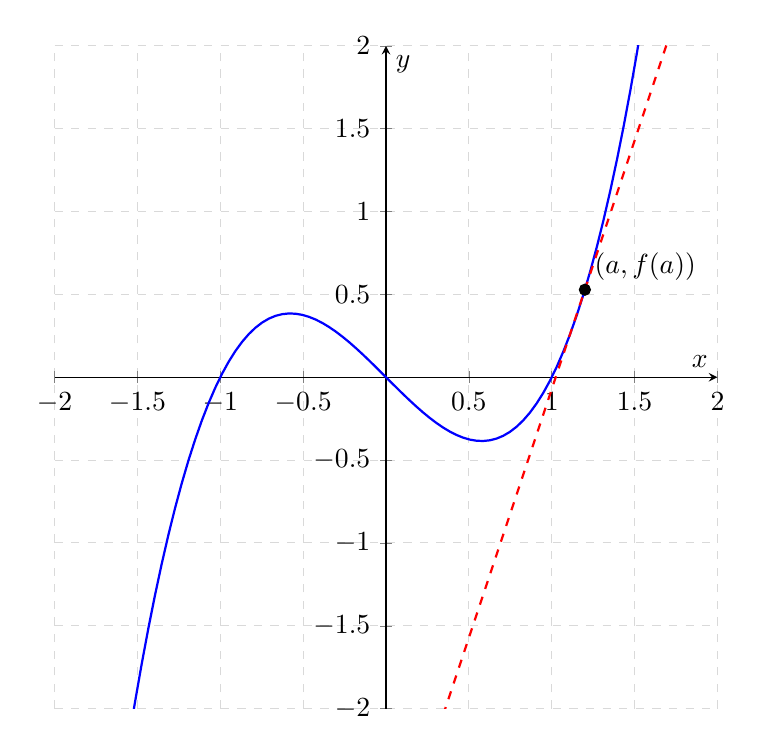
\begin{tikzpicture}
        \begin{axis}[
            axis lines = middle,
            xlabel = $x$,
            ylabel = $y$,
            xmin = -2, xmax = 2,
            ymin = -2, ymax = 2,
            width=10cm,
            height=10cm,
            grid = major,
            grid style = {dashed, gray!30},
            samples=100
        ]
        % Plot of the function
        \addplot[
            domain=-2:2,
            samples=100,
            color=blue,
            thick
        ]
        {x^3 - x};
        
        % Plot of the tangent line at x = 1.2
        \addplot[
            domain=-2:2,
            samples=100,
            color=red,
            thick,
            dashed
        ]
        {(1.2)^3 - 1.2 + 3*(x - 1.2)};
        
        % Mark the point of tangency
        \addplot[
            only marks,
            mark=*,
            color=black
        ]
        coordinates {(1.2, 1.2^3 - 2*1.2 + 1.2)};
        
        % Labels
        \node at (axis cs:1.2, 1.2^3 - 2*1.2 + 1.2) [anchor=south west] {$(a, f(a))$};
        \end{axis}
    \end{tikzpicture}
\end{center}

A way of seeing this is written by the Taylor polynomial:
\[
f(x) = f(a) + M(x - a) + r(|x - a|)
\]

Where $M = f'(a)$ is the slope of the tangent line and $r(|x - a|)$ is the remainder.

If $x \to a$, then $r(|x - a|) \to 0$ but this only guarantees that the function is continuous at $a$.

However, if
\[
\lim_{x \to a} \frac{r(|x - a|)}{|x - a|} = 0
\]

we actually find the existence of the tangent line at $a$.
\[
\frac{f(x) - f(a)}{x - a} = f'(a) + \frac{r(|x - a|)}{x - a}
\]

\subsection{Generalizing to several variables}
\[
z = f(x,y)
\]
We would like to understand the derivative with respect to each variable.

To do so, we use the knowledge of derivatives in 1 variable.

\subsection{Partial derivatives}
Let $f : A \subset \mathbb{R}^N \rightarrow \mathbb{R}$ be a scalar function. And let $x_0 \in A$. The partial derivative of $f$ with respect to the variable $x_i$ at $x_0$ is defined as:
\[
\frac{\partial f}{\partial x_i}(x_0) = \lim_{t \to 0} \frac{f(x_0 + t e_i) - f(x_0)}{t}
\]

Where $e_i$ is the unit vector in the direction of $x_i$.

Somehow, we are computing the ratio of the change of the function $f$ in the direction of $x_i$, in other words, of the vector $e_i$.
\[
e_i = (0, \ldots, 0, 1, 0, \ldots, 0)
\]
\[
B = \{e_1, e_2, \ldots, e_N\} \quad \text{is the standard basis of } \mathbb{R}^N
\]

If $F : \mathbb{R}^N \rightarrow \mathbb{R}^M$ is a vector function, then the partial derivative of $F$ with respect to the variable $x_i$ at the point $x$ is defined as:
\[
\frac{\partial F(x)}{\partial x_i} = \left(\frac{\partial f_1}{\partial x_i}, \frac{\partial f_2}{\partial x_i}, \ldots, \frac{\partial f_M}{\partial x_i}\right)
\]

\subsection*{Example:}
\[
f(x,y) = xy +x - y \quad \text{at } (0,0)
\]

\[
\frac{\partial f}{\partial x}(0,0) = \lim_{t \to 0} \frac{f(0 + t e_1) - f(0,0)}{t} = \lim_{t \to 0} \frac{f(t,0) - f(0,0)}{t} = \lim_{t \to 0} \frac{t \cdot 0 + t - 0}{t} = 1
\]

Where $t$ is the norm of the vector $t e_1$:
\[
t = t ||e_1|| = t \cdot 1 = t
\]

Now, 
\[
\frac{\partial f}{\partial y}(0,0) = \lim_{k \to 0} \frac{f(0,k) - f(0,0)}{t} = \lim_{k \to 0} \frac{0 \cdot k + 0 - k}{k} = -1
\]

\subsection{Geometrical interpretation of the partial derivative}
The partial derivative of a function $f : \mathbb{R}^2 \rightarrow \mathbb{R}$ at a point $(x_0, y_0)$ is the slope of the tangent line to the curve $z = f(x,y)$ at the point $(x_0, y_0)$ in the direction of the variable $x_i$.
\[
\frac{\partial f}{\partial x}(x_0, y_0) = \text{slope of the tangent line in the direction of } x
\]
\[
\frac{\partial f}{\partial y}(x_0, y_0) = \text{slope of the tangent line in the direction of } y
\]

\begin{center}
    \tikzsetnextfilename{surface_tangent_lines}
    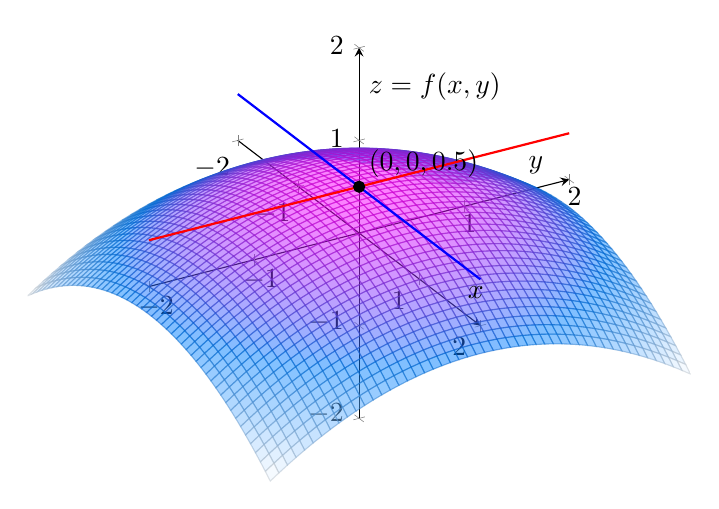
\begin{tikzpicture}
        \begin{axis}[
            axis lines = middle,
            xlabel = $x$,
            ylabel = $y$,
            zlabel = {$z = f(x,y)$},
            xmin = -2, xmax = 2,
            ymin = -2, ymax = 2,
            zmin = -2, zmax = 2,
            width=10cm,
            height=10cm,
            view={60}{30},
            grid = major,
            grid style = {dashed, gray!30},
            samples=50,
            colormap/cool,
        ]
        % Surface
        \addplot3[
            domain=-2:2,
            y domain=-2:2,
            surf,
            opacity=0.5
        ]
        {- (x^2)/5 - (y^2)/5 + 0.5};

        % Point P
        \addplot3[mark=*, color=black] coordinates {(0, 0, 0.5)};

        % Intersection of x = 0 and z = 0
        \addplot3[
            color=red,
            thick
        ]
        coordinates {(0, -2, 0.5) (0, 2, 0.5)};

        % Intersection of y = 0 and z = 0
        \addplot3[
            color=blue,
            thick
        ]
        coordinates {(-2, 0, 0.5) (2, 0, 0.5)};
        
        % Labels
        \node at (axis cs:0, 0, 0.5) [anchor=south west] {$(0, 0, 0.5)$};
        \end{axis}
    \end{tikzpicture}
\end{center}

Obviously, we can apply the rules for derivatives:
\[
\frac{\partial f}{\partial x}(x,y) = y + 1, \quad \frac{\partial f}{\partial y}(x,y) = x - 1
\]

\subsection{Directional derivative}
Let $f : \mathbb{R}^N \rightarrow \mathbb{R}$ be a scalar function and $P \in A \subset \mathbb{R}^N$ and $v \in \mathbb{R}^N$ be a vector. The directional derivative of $f$ at $P$ in the direction of $v$ is defined as:
\[
D_v f(P) = \lim_{t \to 0} \frac{f(P + t v) - f(P)}{t||v||} = \frac{df(P + tv)}{dt} 
\]

\subsection*{Example:}
\[
f(x,y) = \sqrt{|xy|} \quad \text{at } (0,0) \quad \text{in the direction of } v = (1,1)
\]

\[
D_{(1,1)} f(0,0) = \lim_{t \to 0} \frac{f(0 + t, 0 + t) - f(0,0)}{t||(1,1)||} = \lim_{t \to 0} \frac{\sqrt{|t^2|} - 0}{t||(1,1)||} = \lim_{t \to 0} \frac{|t|}{t\sqrt{2}} = 
\begin{cases}
    \dfrac{1}{\sqrt{2}} & \text{if } t \to 0^+ \\
    -\dfrac{1}{\sqrt{2}} & \text{if } t \to 0^-
\end{cases}
\]

Therefore, the directional derivative does not exist.

\subsection{Remark}
Existence of all directional derivatives at a point $P$ does not guarantee the continuity of the function at $P$.
\[
\text{For example: } f(x,y) =
\begin{cases}
    1 & \text{if } x = 0 \text{ or } y = 0 \\
    0 & \text{otherwise}
\end{cases}
\]

\[
\frac{\partial f}{\partial x}(0,0) = 0 = \frac{\partial f}{\partial y}(0,0)
\]
\[
\lim_{(x,y) \to (0,0)} f(x,y) \text{ does not exist.}
\]

\subsection*{Example:}
\[
f(x,y) = x^{1/3}y^{1/3} \quad \text{at } (0,0)
\]

\[
\frac{\partial f}{\partial x}(0,0) = \lim_{t \to 0} \frac{f(t,0) - f(0,0)}{t} = \lim_{t \to 0} \frac{t^{1/3} \cdot 0^{1/3} - 0}{t} = 0
\]

\[
\frac{\partial f}{\partial y}(0,0) = \lim_{t \to 0} \frac{f(0,t) - f(0,0)}{t} = \lim_{t \to 0} \frac{0 \cdot t^{1/3} - 0}{t} = 0
\]

Derivatives exist and the function is also continuous at $(0,0)$. However, there is no tangent plane at $(0,0)$.

\subsection{Differentiability}
Heuristically it means the construction of a tangent plane.

\begin{center}
    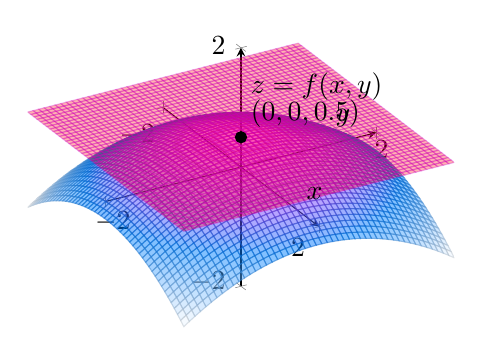
\begin{tikzpicture}
        \begin{axis}[
            axis lines = middle,
            xlabel = $x$,
            ylabel = $y$,
            zlabel = {$z = f(x,y)$},
            xmin = -2, xmax = 2,
            ymin = -2, ymax = 2,
            zmin = -2, zmax = 2,
            width=7cm,
            height=7cm,
            view={60}{30},
            grid = major,
            grid style = {dashed, gray!30},
            samples=50,
            colormap/cool,
        ]
        % Surface
        \addplot3[
            domain=-2:2,
            y domain=-2:2,
            surf,
            opacity=0.5
        ]
        {- (x^2)/5 - (y^2)/5 + 0.5};

        % Tangent plane
        \addplot3[
            domain=-2:2,
            y domain=-2:2,
            surf,
            opacity=0.3,
            color=red
        ]
        {0.5};

        % Point P
        \addplot3[mark=*, color=black] coordinates {(0, 0, 0.5)};
        
        % Labels
        \node at (axis cs:0, 0, 0.5) [anchor=south west] {$(0, 0, 0.5)$};
        \end{axis}
    \end{tikzpicture}
    \hspace{1cm}
    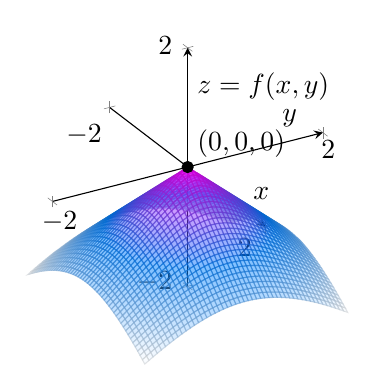
\begin{tikzpicture}
        \begin{axis}[
            axis lines = middle,
            xlabel = $x$,
            ylabel = $y$,
            zlabel = {$z = f(x,y)$},
            xmin = -2, xmax = 2,
            ymin = -2, ymax = 2,
            zmin = -2, zmax = 2,
            width=7cm,
            height=7cm,
            view={60}{30},
            grid = major,
            grid style = {dashed, gray!30},
            samples=50,
            colormap/cool,
        ]
        % Surface with spike
        \addplot3[
            domain=-1.5:1.5,
            y domain=-1.5:1.5,
            surf,
            opacity=0.5
        ]
        {- sqrt(x^2 + y^2)};

        % Point P
        \addplot3[mark=*, color=black] coordinates {(0, 0, 0)};
        
        % Labels
        \node at (axis cs:0, 0, 0) [anchor=south west] {$(0, 0, 0)$};
        \end{axis}
    \end{tikzpicture}
\end{center}

Let $A \subset \mathbb{R}^2$ be an open subset in $\mathbb{R}^2$ such that $(x,y) \in A$, with $f : A \rightarrow \mathbb{R}$ a scalar function. We say that $f$ is differentiable at $(x_0, y_0)$ if: 
\begin{enumerate}
    \item $\dfrac{\partial f}{\partial x}(x_0, y_0)$ and $\dfrac{\partial f}{\partial y}(x_0, y_0)$ exist.
    \item $\lim_{(x,y) \to (x_0, y_0)} \dfrac{f(x,y) - f(x_0, y_0) - \dfrac{\partial f}{\partial x}(x_0, y_0)(x - x_0) - \dfrac{\partial f}{\partial y}(x_0, y_0)(y - y_0)}{\sqrt{(x - x_0)^2 + (y - y_0)^2}} = 0$
\end{enumerate}

To be differentiable we say that there exists a tangent plane at $(x_0, y_0)$:
\[
z = f(x_0, y_0) + A(x - x_0) + B(y - y_0)
\]
Following similar ideas to the 1D case, we can write:
\[
f(x,y) = f(x_0, y_0) + A(x - x_0) + B(y - y_0) + r(\|(x, y) - (x_0,y_0)\|)
\]

If $\|(x, y) - (x_0,y_0)\| \to 0$ then $r(\|(x, y) - (x_0,y_0)\|) \to 0$, and the function is continuous at $(x_0, y_0)$.

However if we have:
\[
\frac{f(x,y) - f(x_0, y_0) - A(x - x_0) - B(y - y_0)}{\|(x - x_0) + (y - y_0)}\| = \frac{r(\|(x, y) - (x_0,y_0)\|)}{\|(x - x_0) + (y - y_0)\|} \to 0
\]

Then the function is differentiable at $(x_0, y_0)$ if:
\[
A = \frac{\partial f}{\partial x}(x_0, y_0), \quad B = \frac{\partial f}{\partial y}(x_0, y_0)
\]

\paragraph{Remark}
Taylor's polynomial around $(x_0, y_0)$ of degree 1 is:
\[
f(x,y) = f(x_0, y_0) + \frac{\partial f}{\partial x}(x_0, y_0)(x - x_0) + \frac{\partial f}{\partial y}(x_0, y_0)(y - y_0) + r(\|(x, y) - (x_0,y_0)\|)
\]
Where $\dfrac{\partial f}{\partial x}(x_0, y_0)$ and $\dfrac{\partial f}{\partial y}(x_0, y_0)$ form $L\left((x - x_0), (y - y_0)\right)$, the linearity function.
\[
\|f(x,y) - L\left((x - x_0), (y - y_0)\right)\| < \varepsilon \text{ as } \|(x, y) - (x_0, y_0)\| < \delta
\]

We can write $L$ in terms of the derivative of the scalar function $f$:
\[
f : \mathbb{R}^2 \rightarrow \mathbb{R} 
\]

We define such a derivative as the gradient of $f$:
\[
D(f(x,y)) = \nabla f(x,y) = \left(\frac{\partial f}{\partial x}, \frac{\partial f}{\partial y}\right)
\]

The gradient provides us with the direction of the maximum increase of the function $f$ at $(x,y)$.

\subsection*{Problem 4a}
\[
f(x,y) = xy, \quad \frac{\partial f}{\partial x} = y, \quad \frac{\partial f}{\partial y} = x
\]

\subsection*{Problem 4c}
\[
f(x,y) = \sqrt{^2 + y^2}, \quad \frac{\partial f}{\partial x} = \frac{x}{\sqrt{x^2 + y^2}}, \quad \frac{\partial f}{\partial y} = \frac{y}{\sqrt{x^2 + y^2}}
\]

\subsection*{Problem 5a}
\[
f(x,y,z) = (x + z) e^{x - y}, \quad \text{gradient at } (1,1,1)
\]
\[
\nabla f(x,y,z) = \left(\frac{\partial f}{\partial x}, \frac{\partial f}{\partial y}, \frac{\partial f}{\partial z}\right) = \left(e^{x - y} + (x + z)e^{x - y}, -(x + z)e^{x - y}, e^{x - y}\right)
\]
\[
\nabla f(1,1,1) = (e^0 + 2e^0, -2e^0, e^0) = (3, -2, 1)
\]

\section{Differentiability in $\mathbb{R}^N$}
\[
A \subset \mathbb{R}^N, \quad x_0 \in A, \quad f : A \rightarrow \mathbb{R}^M
\] 
We say that $f$ is differentiable at $x_0$ if:
\begin{enumerate}
    \item $\dfrac{\partial f_i}{\partial x_j}(x_0)$ exists for $i = 1, 2, \ldots, M$ and $j = 1, 2, \ldots, N$.
    \item $\lim_{x \to x_0} \dfrac{f(x) - f(x_0) - Jf(x_0)(x - x_0)}{||x - x_0||} = 0$
\end{enumerate}
    
Where $Jf(x_0)$ is the Jacobian matrix of $f$ at $x_0$:
\[
Jf(x_0) = Df(x_0) =
\begin{pmatrix}
    \dfrac{\partial f_1}{\partial x_1} & \dfrac{\partial f_1}{\partial x_2} & \ldots & \dfrac{\partial f_1}{\partial x_N} \\
    \dfrac{\partial f_2}{\partial x_1} & \dfrac{\partial f_2}{\partial x_2} & \ldots & \dfrac{\partial f_2}{\partial x_N} \\
    \vdots & \vdots & \ddots & \vdots \\
    \dfrac{\partial f_M}{\partial x_1} & \dfrac{\partial f_M}{\partial x_2} & \ldots & \dfrac{\partial f_M}{\partial x_N}
\end{pmatrix}
\]

\subsection*{Problem 6a}
Compute the jacobian matrix:
\[
F(x,y) = (y,x,xy,y^2 - x^2), \quad F : \mathbb{R}^2 \rightarrow \mathbb{R}^4
\]

\[
JF(x,y) =
\begin{pmatrix}
    \dfrac{\partial y}{\partial x} & \dfrac{\partial y}{\partial y} \\
    \dfrac{\partial x}{\partial x} & \dfrac{\partial x}{\partial y} \\
    \dfrac{\partial xy}{\partial x} & \dfrac{\partial xy}{\partial y} \\
    \dfrac{\partial y^2 - x^2}{\partial x} & \dfrac{\partial y^2 - x^2}{\partial y}
\end{pmatrix} =
\begin{pmatrix}
    0 & 1 \\
    1 & 0 \\
    y & x \\
    -2x & 2y
\end{pmatrix}
\]
Now at $(1,2)$:
\[
JF(1,2) =
\begin{pmatrix}
    0 & 1 \\
    1 & 0 \\
    2 & 1 \\
    -2 & 4
\end{pmatrix}
\]

\subsection*{Problem 6c}
\[
F(x,y,z) = z^2 e^x \cos(y), \text{ at } (0, \frac{\pi}{2}, -1) \quad F : \mathbb{R}^3 \rightarrow \mathbb{R}
\]

\[
JF(x,y,z) =
\begin{pmatrix}
    \dfrac{\partial z^2 e^x \cos(y)}{\partial x} & \dfrac{\partial z^2 e^x \cos(y)}{\partial y} & \dfrac{\partial z^2 e^x \cos(y)}{\partial z}
\end{pmatrix} =
\]
\[
= 
\begin{pmatrix}
    z^2 e^x \cos(y) & -z^2 e^x \sin(y) & 2z e^x \cos(y)
\end{pmatrix}
\]

\[
JF(0, \frac{\pi}{2}, -1) =
\begin{pmatrix}
    0 & -1 & 0
\end{pmatrix}
\]

\subsection*{Example:}
\[
f(x,y) = 
\begin{cases}
    \dfrac{2xy}{\sqrt{x^2 + y^2}} & \text{if } (x,y) \neq (0,0) \\
    0 & \text{if } (x,y) = (0,0)
\end{cases}
\]

$f$ is not differentiable at $(0,0)$, the partial derivatives exist at $(0,0)$.
\[
\frac{\partial f}{\partial x}(0,0) = \lim_{t \to 0} \frac{f(t,0) - f(0,0)}{t} = \lim_{t \to 0} \frac{2t \cdot 0}{t \cdot 0} = 0
\]
\[
\frac{\partial f}{\partial y}(0,0) = \lim_{t \to 0} \frac{f(0,t) - f(0,0)}{t} = \lim_{t \to 0} \frac{2 \cdot 0 \cdot t}{t \cdot 0} = 0
\]

However, the limit of the difference quotient does not exist:
\[
\lim_{(x,y) \to (0,0)} \frac{f(x,y) - f(0,0) - \frac{\partial f}{\partial x}(0,0)x - \frac{\partial f}{\partial y}(0,0)y}{\sqrt{x^2 + y^2}} =
\]

\[
= \lim_{(x,y) \to (0,0)} \dfrac{\dfrac{2xy}{\sqrt{x^2 + y^2}} - 0 - 0 \cdot x - 0 \cdot y}{\sqrt{x^2 + y^2}} = \lim_{(x,y) \to (0,0)} \frac{2xy}{x^2 + y^2}
\]

If we use polar coordinates:
\[
\begin{cases}
    x = r \cos(\theta) \\
    y = r \sin(\theta)
\end{cases}
\]

\[
= \lim_{r \to 0} \frac{2r^2 \cos(\theta) \sin(\theta)}{r^2} = \lim_{r \to 0} 2 \cos(\theta) \sin(\theta) = 2 \cos(\theta) \sin(\theta)
\]

The limit depends on $\theta$. Therefore, the function is not differentiable at $(0,0)$.

\subsection*{Problem 7}
\[
f(x,y) = 
\begin{cases}
    \dfrac{xy^2}{x^2 + y^4} & \text{if } x \neq 0 \\
    0 & \text{if } x = 0
\end{cases}
\]

The partial derivatives exist at $(0,0)$:
\[
\frac{\partial f}{\partial x}(0,0) = \lim_{t \to 0} \frac{f(t,0) - f(0,0)}{t} = \lim_{t \to 0} \frac{0 - 0}{t} = 0
\]
\[
\frac{\partial f}{\partial y}(0,0) = \lim_{t \to 0} \frac{f(0,t) - f(0,0)}{t} = \lim_{t \to 0} \frac{0 - 0}{t} = 0
\]

Take the limit:
\[
\lim_{(x,y) \to (0,0)} f(x,y) = \lim_{(x,y) \to (0,0)} \frac{xy^2}{x^2 + y^4} = lim_{r \to 0} \frac{r^3 \cos(\theta) \sin^2(\theta)}{r^2 \cos^2(\theta) + r^4 \sin^4(\theta)}
\]

The limit does not exist, therefore the function is not continuous at $(0,0)$. The function is not differentiable at $(0,0)$, due to it not being continuous at that point.

Direction of any vector at $(0,0)$:
\[
D_(u,v) f(0,0) = \lim_{t \to 0} \frac{f(tu, tv) - f(0,0)}{t \|(u,v)\|}
\]

Assume $\|(u,v)\| = 1$:
\[
= \lim_{t \to 0} \frac{f(tu, tv)}{t} = \lim_{t \to 0} \frac{t^3 u v^2}{t(t^2 u^2 + t^4 v^4)} = \lim_{t \to 0} \frac{u v^2}{u^2 + t^2 v^4} = \frac{v^2}{u}
\]

Where $\dfrac{v^2}{u}$ is the slope of the tangent line in the direction of $(u,v)$.

\subsection{Proposition:}
\[
A \subset \mathbb{R}^N, \quad x_0 \in A, \quad f : A \rightarrow \mathbb{R}
\]

$f$ is a scalar function, differentiable at $x_0$ and $v \in \mathbb{R}^N \backslash 0$ a vector. Then:
\[
D_v f(x_0) = \inner{\nabla f(x_0)}{v}
\]

\paragraph{Remark}
\[
\inner{\nabla f(x_0)}{\alpha v} = \alpha \inner{\nabla f(x_0)}{v} \neq \inner{\nabla f(x_0)}{v}
\]

Using the properties of the scalar product: 
\[
D_v f(x_0) = \inner{\nabla f(x_0)}{v} = ||\nabla f(x_0)|| \cdot ||v|| \cdot \cos(\theta) = ||\nabla f(x_0)|| \cdot \cos(\theta)
\]

Where $\theta$ is the angle between $\nabla f(x_0)$ and $v$, and we assume $\|v\| = 1$.

The directional derivative is maximum in the direction of $\nabla f(x_0)$ and minimum in the direction of $-\nabla f(x_0)$.

\subsection{Proposition:}
Let \( f: \mathbb{R}^3 \rightarrow \mathbb{R} \) be a scalar function and let \((x_0, y_0, z_0) \in \mathbb{R}^3\) be a point on the level surface \(\{ f(x, y, z) = k \in \mathbb{R} \} = S\).

Then, \( \nabla f(x_0, y_0, z_0) \perp v = 0 \) where \(v\) is the tangent vector to the trajectory \(c(t)\) at \(t = 0\) over the surface \(S\).

\subsection*{Proof}
Since \(c(t) \subset S\), we have \(f(c(t)) = k\).

By construction, \(v = c'(0)\).

Now, applying the chain rule, we get:
\[
\frac{d}{dt} f(c(t)) \bigg|_{t=0} = \nabla f(c(0)) \cdot c'(0) = \nabla f(c(0)) \cdot v = 0
\]

This proves the orthogonality between \(\nabla f\) and the tangent vector to the curve (to the level curve).

\subsection*{Remark}
Take \(P^* (p_1, p_2, p_3)\) as a point and \((x, y, z)\) as any point on the tangent plane.

Then,
\[
n \cdot (x - p_1, y - p_2, z - p_3) = 0
\]

where \(n = \nabla f(P^*)\).

\subsection{Tangent Plane to a Surface}

The tangent plane to \( f(x, y, z) = k \) at \( p_0 \) is given by

\[
\nabla f(p_0) \cdot
\begin{pmatrix}
x - p_1 \\
y - p_2 \\
z - p_3
\end{pmatrix}
= 0
\]

\begin{multicols}{2}
    \subsection*{Example}
    \textbf{Tangent plane of \( 3xy + z^2 = 4 \) at \((1, 1, 1)\):}
    \begin{itemize}
        \item \textbf{Gradient:} \\
        \( \nabla f(x, y, z) = (3x, 3y, 2z) \)
        \item \textbf{Gradient at (1, 1, 1):} \\
        \( \nabla f(1, 1, 1) = (3, 3, 2) \)
        \item \textbf{Tangent Plane:} \\
        \( \nabla f(1, 1, 1) \cdot \begin{pmatrix}
        x - 1 \\
        y - 1 \\
        z - 1
        \end{pmatrix} = 0 \)
        \item \textbf{Equation:} \\
        \( 3(x - 1) + 3(y - 1) + 2(z - 1) = 0 \) \\
        \( 3x + 3y + 2z = 8 \)
    \end{itemize}
\columnbreak
    \subsection*{Problem 11c}
    \textbf{Find the tangent plane of \( z = \dfrac{x}{y^2} \) at \((-2, 2, 1)\):}
    \begin{itemize}
        \item \textbf{Gradient:} \\
        \( \nabla f(x, y, z) = \left(\dfrac{1}{y^2}, -\dfrac{2x}{y^3}, -1\right) \)
        \item \textbf{Gradient at (-2, 2, 1):} \\
        \( \nabla f(-2, 2, 1) = \left(\dfrac{1}{4}, -\dfrac{1}{2}, -1\right) \)
        \item \textbf{Tangent Plane:} \\
        \( \nabla f(-2, 2, 1) \cdot \begin{pmatrix}
        x + 2 \\
        y - 2 \\
        z - 1
        \end{pmatrix} = 0 \)
        \item \textbf{Equation:} \\
        \( \dfrac{1}{4}(x + 2) - \dfrac{1}{2}(y - 2) - (z - 1) = 0 \) \\
        \( \dfrac{1}{4}x - \dfrac{1}{2}y - z = -\dfrac{1}{2} \)
    \end{itemize}
\end{multicols}

\subsection{Theorems}
Let \( A \subseteq \mathbb{R}^n \), \( x_0 \in A \), and \( f: A \subseteq \mathbb{R}^n \rightarrow \mathbb{R}^m \). If \( f \) is differentiable at \( x_0 \), \( f \) is continuous at \( x_0 \).


Let \( A \subseteq \mathbb{R}^n \), \( x_0 \in A \), and \( f: A \subseteq \mathbb{R}^n \rightarrow \mathbb{R} \). For \( x = (x_1, \ldots, x_n) \):
\begin{itemize}
    \item[a)] \( \dfrac{\partial f}{\partial x_i} \) exists for any \( i \).
    \item[b)] \( \dfrac{\partial f}{\partial x_i} \) is continuous at \( x_0 \) for any \( i \).
\end{itemize}
Then, \( f \) is differentiable at \( x_0 \).

\subsection*{Problem 9}
Given \( f(x,y) = e^{\left(\dfrac{1}{x^2 + y^2}\right)} \) for \( (x,y) \neq (0,0) \) and \( f(0,0) = 0 \):
\begin{itemize}
    \item[a)] Show that \( f \) is differentiable at \( (0,0) \).
    \item[b)] Prove the existence of the tangent plane at \( (0,0) \).
\end{itemize}

To show \( f \) is differentiable at \( (0,0) \), we need to check the limit:
\[
\lim_{(x,y) \to (0,0)} \frac{f(x,y) - f(0,0) - \frac{\partial f}{\partial x}(0,0)x - \frac{\partial f}{\partial y}(0,0)y}{\sqrt{x^2 + y^2}} = 0
\]

\[
\dfrac{\partial f}{\partial x} (0,0) = \lim_{t \to 0} \frac{f(t,0) - f(0,0)}{t} = \lim_{t \to 0} \frac{e^{\left(\dfrac{-1}{t^2}\right)}}{t} = 0 = \frac{\partial f}{\partial y} (0,0)
\]

Thus, \( f \) is differentiable at \( (0,0) \).

\subsection{Properties}

Let \( A, B \subseteq \mathbb{R}^n \), \( x_0 \in A \), and \( f, g : A \subseteq \mathbb{R}^n \rightarrow \mathbb{R}^m \) be differentiable functions.

\begin{enumerate}
    \item \( \lambda f(x) \) is differentiable at \( x_0 \), where \( \lambda \in \mathbb{R} \). The derivative is given by:
    
    \[
    D(\lambda f(x_0)) = \lambda D(f(x_0))
    \]

    \item \( f(x) + g(x) \) is differentiable at \( x_0 \). The derivative is given by:

    \[
    D(f(x_0) + g(x_0)) = D(f(x_0)) + D(g(x_0))
    \]

    \item \( f(x) \cdot g(x) \) is differentiable at \( x_0 \). The derivative is given by:
    
    \[
    D(f(x_0) \cdot g(x_0)) = D(f(x_0)) \cdot g(x_0) + f(x_0) \cdot D(g(x_0))
    \]

    \item \( \dfrac{f(x)}{g(x)} \) is differentiable at \( x_0 \), provided \( g(x_0) \neq 0 \). The derivative is given by:
    
    \[
    D\left( \frac{f(x_0)}{g(x_0)} \right) = \frac{D(f(x_0)) \cdot g(x_0) - f(x_0) \cdot D(g(x_0))}{(g(x_0))^2}
    \]

\end{enumerate}

\subsection{Chain Rule}

Let \( f : \mathbb{R}^m \rightarrow \mathbb{R}^n \) and \( g : \mathbb{R}^n \rightarrow \mathbb{R}^k \). If \( x_0 \in \mathbb{R}^m \) and \( f(x_0) \in \mathbb{R}^n \), then \( (g \circ f)(x) = g(f(x)) \) is differentiable at \( x_0 \). The derivative is given by:
\[
D(g \circ f)(x_0) = Dg(f(x_0)) \cdot Df(x_0)
\]

\subsection*{Example}
Given \( g(x, y) = (x^2 + y, y^2) \) and \( F(u, v) = (u + v, u, v^2) \), find \( D(F \circ g)(1, 1) \).

\begin{align*}
g : & \mathbb{R}^2 \rightarrow \mathbb{R}^2 \\
f : & \mathbb{R}^2 \rightarrow \mathbb{R}^3
\end{align*}

\[
g(x, y) = (x^2 + 1, y^2)
\]
\[
f(x, y) = (u + v, u, v^2)
\]

\[
(x, y) \rightarrow \left(g_1(x,y), g_2(x,y)\right) \rightarrow \left(f_1(g_1, g_2), f_2(g_1, g_2), f_3(g_1, g_2)\right)
\]

\[
f(g_1(x,y), g_2(x,y)) = (x^2 + 1 + y^2, x^2 + 1, y^4) \rightarrow Df(x, y) = Jf(x, y)
\]

\[
Dg(x, y) = Jg(x, y) = \begin{pmatrix}
2x & 0 \\
0 & 2y
\end{pmatrix}
\]

\[
Df(u, v) = Jf(u, v) = \begin{pmatrix}
1 & 1 \\
1 & 0 \\
0 & 2v
\end{pmatrix}
\]

\[
D(f \circ g)(x, y) = D(f(g(x, y))) \cdot Dg(x, y) = \begin{pmatrix}
1 & 1 \\
1 & 0 \\
0 & 2v
\end{pmatrix} \cdot \begin{pmatrix}
2x & 0 \\
0 & 2y
\end{pmatrix}
\]

\[
D(F \circ g)(1, 1) = \begin{pmatrix}
1 & 1 \\
1 & 0 \\
0 & 2
\end{pmatrix} \cdot \begin{pmatrix}
2 & 0 \\
0 & 2
\end{pmatrix}
\]

\[
D(F \circ g)(1, 1) = \begin{pmatrix}
2 & 2 \\
2 & 0 \\
0 & 4
\end{pmatrix}
\]

\subsection*{Example}
\( f(x,y) = \left( \tan \dfrac{y}{x} - x + y, \log \dfrac{y+1}{x} \right) \), \( g(s,t) = \left( t \cdot \cos s, e^t, s - 2t \right) \) and \( h(u, v, w) = uv^2 \cdot e^w \)

\[
F = h \circ g \circ f
\]
\[
DF(x, y) = D(h(g(f)(x, y))) \cdot D(g(f(x, y))) \cdot D(f(x, y))
\]

\[
Df(x, y) = \begin{pmatrix}
-\dfrac{sec^2 \dfrac{y}{x} \cdot y}{x^2} - 1 & \dfrac{sec^2 \dfrac{y}{x}}{x} + 1 \\
-\dfrac{1}{x} & \dfrac{1}{y+1}
\end{pmatrix}
\]

\[
Dg(s, t) = \begin{pmatrix}
-t \cdot \sin s & \cos s \\
0 & e^t \\
1 & -2
\end{pmatrix}
\]

\[
Dh(u, v, w) = \begin{pmatrix}
v^2 \cdot e^w & 2uv \cdot e^w & uv^2 \cdot e^w
\end{pmatrix}
\]

\subsection*{Example}

Particle of mass $m$ following a trajectory $s(t) \in \mathbb{R}^3$

According to Newton's law, the field force satisfies
\[ F = -\nabla V \quad \text{with} \quad V = \text{potential function} \]

Prove that the total energy is constant $E(t) = E_k + E_p = c$

Following $s(t)$ we find $F(s(t)) = -\nabla V(s(t))$

Taking the arbitrary times $t_1, t_2$
\[ \int_{t_1}^{t_2} F(s(t)) \cdot d(s(t)) = -\int_{t_1}^{t_2} \nabla V(s(t)) \cdot s'(t) \, dt \quad \text{(chain rule)} \]

\[ -\left( V(s(t_2)) - V(s(t_1)) \right) \]

Thanks to Newton's second law
\[ F = m \, s''(t) \]

\[ \int_{t_1}^{t_2} F(s(t)) \cdot s'(t) \, dt = \int_{t_1}^{t_2} m \, s''(t) \cdot s'(t) \, dt = \left[ \frac{m \| s'(t) \|^2}{2} \right]_{t_1}^{t_2} \]

\[ = \frac{m \| s'(t_2) \|^2}{2} - \frac{m \| s'(t_1) \|^2}{2} \]

\[ E(t) = \frac{m \| s'(t) \|^2}{2} + V(s(t)) \]

\subsection*{Example}
$$ f(x,y) = \begin{cases} \dfrac{2xy}{2x^2 + y^2} & (x,y) \neq (0,0) \\ 0 & (x,y) = (0,0) \end{cases} $$

Partial Derivatives: $$ \frac{\partial f(x,y)}{\partial x} = \lim_{t \to 0} \frac{f(t,0) - f(0,0)}{t} = 0 $$ $$ \frac{\partial f(x,y)}{\partial y} = \lim_{k \to 0} \frac{f(0,k) - f(0,0)}{k} = 0 $$

Differentiability at (0,0): $$ \lim_{(x,y) \to (0,0)} \frac{\dfrac{2xy}{2x^2 + y^2}}{\sqrt{x^2 + y^2}} = \lim_{(x,y) \to (0,0)} \frac{2xy}{\sqrt{x^2 + y^2} \left(2x^2 + y^2\right)} $$ $$ \begin{cases}x = r \cos \theta \\ y = r \sin \theta \end{cases}$$ $$ \lim_{r \to 0} \frac{2 \cos \theta \sin \theta}{r \left(2 \cos^2 \theta + \sin^2 \theta\right)} = \infty \quad f \text{ is not differentiable at } (0,0) $$

Directional derivative following $v = \left(\frac{1}{\sqrt{2}}, \frac{1}{\sqrt{2}}\right)$:

$$ \text{Using } D_v f(0, 0) = \inner{\nabla f(0, 0)}{v} = \inner{\left(0, 0\right)}{\left(\frac{1}{\sqrt{2}}, \frac{1}{\sqrt{2}}\right)} = 0 $$
$$ D_v f(0, 0) = \lim_{t \to 0} \frac{f(0, 0) + tv) - f(0, 0)}{t} = \lim_{t \to 0} \frac{f(tv) - f(0, 0)}{t} = \lim_{t \to 0} \frac{\dfrac{2t^2}{2}}{\dfrac{2t^2}{2} + \dfrac{t^2}{2}} = \frac{2}{3} $$


\subsection*{Problem 17}
Use a tree diagram to write out the Chain Rule for the given case. Assume all functions
are differentiable.
\[
\mathbf{a)} \quad u = f(x, y), \quad x = x(r, s, t), \quad y = y(r, s, t)
\]
\[
(r, s, t) \rightarrow (x(r, s, t), y(r, s, t)) \rightarrow f(x(r, s, t), y(r, s, t))
\]
\[
\mathbb{R}^3 \rightarrow \mathbb{R}^2 \rightarrow \mathbb{R}
\]

\[
D(f \circ g)(r, s, t) = D(f(g(r, s, t))) \cdot Dg(r, s, t)
\]
\[
D(f \circ g)(r, s, t) = Df(x(r, s, t), y(r, s, t)) \cdot \begin{pmatrix}
    \dfrac{\partial x}{\partial r} & \dfrac{\partial x}{\partial s} & \dfrac{\partial x}{\partial t} \\
    \dfrac{\partial y}{\partial r} & \dfrac{\partial y}{\partial s} & \dfrac{\partial y}{\partial t}
\end{pmatrix}
\]
\[
D(f \circ g)(r, s, t) = \begin{pmatrix}
    \dfrac{\partial f}{\partial x} & \dfrac{\partial f}{\partial y}
\end{pmatrix} \cdot \begin{pmatrix}
    \dfrac{\partial x}{\partial r} & \dfrac{\partial x}{\partial s} & \dfrac{\partial x}{\partial t} \\
    \dfrac{\partial y}{\partial r} & \dfrac{\partial y}{\partial s} & \dfrac{\partial y}{\partial t}
\end{pmatrix}
\]
\[
D(f \circ g)(r, s, t) = \begin{pmatrix}
    \dfrac{\partial f}{\partial x} \cdot \dfrac{\partial x}{\partial r} + \dfrac{\partial f}{\partial y} \cdot \dfrac{\partial y}{\partial r} & \dfrac{\partial f}{\partial x} \cdot \dfrac{\partial x}{\partial s} + \dfrac{\partial f}{\partial y} \cdot \dfrac{\partial y}{\partial s} & \dfrac{\partial f}{\partial x} \cdot \dfrac{\partial x}{\partial t} + \dfrac{\partial f}{\partial y} \cdot \dfrac{\partial y}{\partial t}
\end{pmatrix}
\]

\[ \mathbf{b)} \quad w = f(x, y, z), \quad x = x(u, v), \quad y = y(u, v), \quad z = z(u, v) \]
\[ (u, v) \rightarrow (x(u, v), y(u, v), z(u, v)) \rightarrow f(x(u, v), y(u, v), z(u, v)) \]
\[ \mathbb{R}^2 \rightarrow \mathbb{R}^3 \rightarrow \mathbb{R} \]

\[ D(f \circ g)(u, v) = D(f(g(u, v))) \cdot Dg(u, v) \]
\[ D(f \circ g)(u, v) = Df(x(u, v), y(u, v), z(u, v)) \cdot \begin{pmatrix}
    \dfrac{\partial x}{\partial u} & \dfrac{\partial x}{\partial v} \\
    \dfrac{\partial y}{\partial u} & \dfrac{\partial y}{\partial v} \\
    \dfrac{\partial z}{\partial u} & \dfrac{\partial z}{\partial v}
\end{pmatrix} \]
\[ D(f \circ g)(u, v) = \begin{pmatrix}
    \dfrac{\partial f}{\partial x} & \dfrac{\partial f}{\partial y} & \dfrac{\partial f}{\partial z}
\end{pmatrix} \cdot \begin{pmatrix}
    \dfrac{\partial x}{\partial u} & \dfrac{\partial x}{\partial v} \\
    \dfrac{\partial y}{\partial u} & \dfrac{\partial y}{\partial v} \\
    \dfrac{\partial z}{\partial u} & \dfrac{\partial z}{\partial v}
\end{pmatrix} \]
\[ D(f \circ g)(u, v) = \begin{pmatrix}
    \dfrac{\partial f}{\partial x} \big|_{g(u, v)} \cdot \dfrac{\partial x}{\partial u} + \dfrac{\partial f}{\partial y} \big|_{g(u, v)} \cdot \dfrac{\partial y}{\partial u} + \dfrac{\partial f}{\partial z} \big|_{g(u, v)} \cdot \dfrac{\partial z}{\partial u} \\
    \dfrac{\partial f}{\partial x} \big|_{g(u, v)} \cdot \dfrac{\partial x}{\partial v} + \dfrac{\partial f}{\partial y} \big|_{g(u, v)} \cdot \dfrac{\partial y}{\partial v} + \dfrac{\partial f}{\partial z} \big|_{g(u, v)} \cdot \dfrac{\partial z}{\partial v}
\end{pmatrix}^t \]

\subsection*{Problem 12}

Let \( f : \mathbb{R}^3 \rightarrow \mathbb{R} \) be differentiable. Making the transformation to spherical coordinates, compute \(\frac{\partial f}{\partial \rho}\), \(\frac{\partial f}{\partial \theta}\), and \(\frac{\partial f}{\partial \phi}\) in terms of \(\frac{\partial f}{\partial x}\), \(\frac{\partial f}{\partial y}\), and \(\frac{\partial f}{\partial z}\).

The transformation to spherical coordinates is given by:
\[
\begin{cases}
x = \rho \sin(\phi) \cos(\theta) \\
y = \rho \sin(\phi) \sin(\theta) \\
z = \rho \cos(\phi)
\end{cases}
\]

\[
(\rho, \theta, \phi) \rightarrow (x(\rho, \theta, \phi), y(\rho, \theta, \phi), z(\rho, \theta, \phi)) \rightarrow f(x(\rho, \theta, \phi), y(\rho, \theta, \phi), z(\rho, \theta, \phi))
\]

\[
\frac{\partial f}{\partial \rho} = \frac{\partial f}{\partial x} \cdot \frac{\partial x}{\partial \rho} + \frac{\partial f}{\partial y} \cdot \frac{\partial y}{\partial \rho} + \frac{\partial f}{\partial z} \cdot \frac{\partial z}{\partial \rho} = \frac{\partial f}{\partial x} \cdot \sin(\phi) \cos(\theta) + \frac{\partial f}{\partial y} \cdot \sin(\phi) \sin(\theta) + \frac{\partial f}{\partial z} \cdot \cos(\phi)
\]
\[
\frac{\partial f}{\partial \theta} = \frac{\partial f}{\partial x} \cdot \frac{\partial x}{\partial \theta} + \frac{\partial f}{\partial y} \cdot \frac{\partial y}{\partial \theta} + \frac{\partial f}{\partial z} \cdot \frac{\partial z}{\partial \theta} = -\frac{\partial f}{\partial x} \cdot \rho \sin(\phi) \sin(\theta) + \frac{\partial f}{\partial y} \cdot \rho \sin(\phi) \cos(\theta)
\]
\[
\frac{\partial f}{\partial \phi} = \frac{\partial f}{\partial x} \cdot \frac{\partial x}{\partial \phi} + \frac{\partial f}{\partial y} \cdot \frac{\partial y}{\partial \phi} + \frac{\partial f}{\partial z} \cdot \frac{\partial z}{\partial \phi} = \frac{\partial f}{\partial x} \cdot \rho \cos(\phi) \cos(\theta) + \frac{\partial f}{\partial y} \cdot \rho \cos(\phi) \sin(\theta) - \frac{\partial f}{\partial z} \cdot \rho \sin(\phi)
\]

\section{Linearization}
\[
\text{Recall:   if } \exists \hspace{0.3cm} \frac{\partial f}{\partial x}, \quad \text{then } \exists \hspace{0.3cm} \frac{\partial f}{\partial y}
\]

\[
\lim_{(h_1,h_2) \to (x_0, y_0)} \frac{f(x,y) - f(x_0, y_0) - \frac{\partial f}{\partial x} \big|_{(x_0, y_0)} h_1 - \frac{\partial f}{\partial y} \big|_{(x_0, y_0)} h_2}{\sqrt{h_1^2 + h_2^2}} = 0
\]

With \( h_1 = x - x_0 \) and \( h_2 = y - y_0 \), we have:
\[
\lim_{(x,y) \to (x_0, y_0)} \frac{f(x,y) - f(x_0, y_0) - \frac{\partial f}{\partial x} \big|_{(x_0, y_0)} (x - x_0) - \frac{\partial f}{\partial y} \big|_{(x_0, y_0)} (y - y_0)}{\sqrt{(x - x_0)^2 + (y - y_0)^2}} = 0
\]

\[
f : \mathbb{R}^n \rightarrow \mathbb{R}^m \quad \text{is differentiable at } x_0 \in \mathbb{R}^n
\]

\[
\lim_{h \to 0} \frac{f(x_0 + h) - f(x_0) - Df\big|_{x_0} \cdot h}{\| h \|} = 0
\]

With $h \in \mathbb{R}^n$, $\quad h = t \cdot v$, $t \to 0 \implies h \to 0$
\[
\lim_{t \to 0} \frac{f(x_0 + t \cdot v) - f(x_0) - Df\big|_{x_0} \cdot t \cdot v}{t} = 0
\]

With $\|v\| = 1$ and $\|h\| = t$

\subsection{Proposition}
If $f : U \subset \mathbb{R}^n \rightarrow \mathbb{R}^m$, $U$ open in $\mathbb{R}^n$ is differentiable at $x_0 \in U$, then $f$ is continuous at $x_0$, then all the directional derivatives exist at $x_0$.
\[
D_v f(x_0) = Df \cdot v = Jf \cdot v
\]

\paragraph{Proof}
\[
v \in \mathbb{R}^n, \quad D_v f = \lim_{t \to 0} \frac{f(x_0 + t \cdot v) - f(x_0)}{t} = \lim_{t \to 0} \frac{Df \big|_{x_0} \cdot t \cdot v}{t} = Df \big|_{x_0} \cdot v
\]

\subsection{Special cases}
\[
f : \mathbb{R}^n \rightarrow \mathbb{R}, \quad \text{differentiable at } x_0, \text{ scalar function}
\]
\[
D_v f = \nabla f = \begin{pmatrix}
    \dfrac{\partial f}{\partial x_1} \\
    \vdots \\
    \dfrac{\partial f}{\partial x_n}
\end{pmatrix}^t \cdot \begin{pmatrix}
    v_1 \\
    \vdots \\
    v_n
\end{pmatrix} = \dfrac{\partial f}{\partial x_1} \cdot v_1 + \ldots + \dfrac{\partial f}{\partial x_n} \cdot v_n
= \inner{\nabla f}{v}
\]

\[
f : \mathbb{R}^2 \rightarrow \mathbb{R}
\]
\[
D_{(1,0)} f = \begin{pmatrix}
    \dfrac{\partial f}{\partial x} \\
    \dfrac{\partial f}{\partial y}
\end{pmatrix}^t \cdot \begin{pmatrix}
    1 \\
    0
\end{pmatrix} = \dfrac{\partial f}{\partial x}
\]

\[
D_{(0,1)} f = \begin{pmatrix}
    \dfrac{\partial f}{\partial x} \\
    \dfrac{\partial f}{\partial y}
\end{pmatrix}^t \cdot \begin{pmatrix}
    0 \\
    1
\end{pmatrix} = \dfrac{\partial f}{\partial y}
\]

\[
D_{v_1, v_2} f = \begin{pmatrix}
    \dfrac{\partial f}{\partial x} \\
    \dfrac{\partial f}{\partial y}
\end{pmatrix}^t \cdot \begin{pmatrix}
    v_1 \\
    v_2
\end{pmatrix} = \dfrac{\partial f}{\partial x} \cdot v_1 + \dfrac{\partial f}{\partial y} \cdot v_2
\]
\[ v_1 + v_2 = 1 \]

\[
f : \mathbb{R}^n \rightarrow \mathbb{R}^m
\]
\[
D_{(1,0, \ldots, 0)} f = \begin{pmatrix}
    \dfrac{\partial f_1}{\partial x_1} \\
    \vdots \\
    \dfrac{\partial f_m}{\partial x_1}
\end{pmatrix}^t \cdot \begin{pmatrix}
    1 \\
    0 \\
    \vdots \\
    0
\end{pmatrix} = \begin{pmatrix}
    \dfrac{\partial f_1}{\partial x_1} \\
    \vdots \\
    \dfrac{\partial f_m}{\partial x_1}
\end{pmatrix}
\]

\[
D_{(0,1, \ldots, 0)} f = \begin{pmatrix}
    \dfrac{\partial f_1}{\partial x_1} \\
    \vdots \\
    \dfrac{\partial f_m}{\partial x_1}
\end{pmatrix}^t \cdot \begin{pmatrix}
    0 \\
    1 \\
    \vdots \\
    0
\end{pmatrix} = \begin{pmatrix}
    \dfrac{\partial f_1}{\partial x_2} \\
    \vdots \\
    \dfrac{\partial f_m}{\partial x_2}
\end{pmatrix}
\]

\subsection{Mean Value Theorem}
\[
f(b) - f(a) = f'(c) \cdot (b - a)
\]

In vectorial calculus, the mean value theorem is only for scalar functions.

\paragraph{Theorem}
Let $U \subset \mathbb{R}^n$ be open, $f : U \rightarrow \mathbb{R}$ be differentiable, and $[a,b] \subset U$. Then, $\forall x \in (a,b)$, $\exists c \in (a,b)$ such that
\[
f(b) - f(a) = Df \big|_c \cdot (b - a) = \nabla f \big|_c \cdot (b - a)
\]

\paragraph{Proof}
We need to use the chain rule:
\[
(1 - t) \cdot a + t \cdot b, \quad t \in [0,1], \quad [0,1] \rightarrow U
\]
\[
g(t) = f((1 - t) \cdot a + t \cdot b)
\]

We apply the mean value theorem for one variable in $[0,1]$:
\[
g(1) - g(0) = g'(t_0) \cdot (1 - 0)
\]

\[
g'(c) = Df \big|_{(1 - t_0) \cdot a + t_0 \cdot b} \cdot (b - a)
\]

Let $c = (1 - t_0) \cdot a + t_0 \cdot b$, then:
\[
f(b) - f(a) = Df \big|_c \cdot (b - a) = \nabla f \big|_c \cdot (b - a)
\]

\subsection{Theorem}
If $U \subset \mathbb{R}^n$ is open, $f : U \rightarrow \mathbb{R}^m$ and all the partial derivatives exist and are continuous on a point $a$, then $f$ is differentiable at $a$ and $Df \big|_a = Jf \big|_a$.

\subsection*{Example}
\[
f(x,y) = 
\begin{cases}
    (x^4 + y^4) \cdot \sin \left( \dfrac{1}{x^4 + y^4} \right) & (x,y) \neq (0,0) \\
    0 & (x,y) = (0,0)
\end{cases}
\]
Is $f$ continuous at $(0,0)$?

\[
\left| sin \left( \dfrac{1}{x^4 + y^4} \right) \right| \leq 1, \quad \text{is bounded}
\]

\[
\implies \exists \hspace{0.3cm} \lim_{(x,y) \to (0,0)} (x^4 + y^4) \cdot \sin \left( \dfrac{1}{x^4 + y^4} \right) = 0
\]

\[
\frac{\partial f}{\partial x} \big|_{(0,0)} = \lim_{h \to 0} \frac{f(h,0) - f(0,0)}{h} = \lim_{h \to 0} \frac{h^4 \cdot \sin \left( \dfrac{1}{h^4} \right)}{h} = 0
\]

\[
\frac{\partial f}{\partial y} \big|_{(0,0)} = \lim_{k \to 0} \frac{f(0,k) - f(0,0)}{k} = \lim_{k \to 0} \frac{k^4 \cdot \sin \left( \dfrac{1}{k^4} \right)}{k} = 0
\]

\[
\implies f \text{ is continuous at } (0,0)
\]

Is $f$ differentiable at $(0,0)$?

\[
\lim_{(x,y) \to (0,0)} \frac{f(x,y) - f(0,0) - \frac{\partial f}{\partial x} \big|_{(0,0)} x - \frac{\partial f}{\partial y} \big|_{(0,0)} y}{\sqrt{x^2 + y^2}} = 
\]
\[
= \lim_{(x,y) \to (0,0)} \frac{(x^4 + y^4) \cdot \sin \left( \dfrac{1}{x^4 + y^4} \right) - 0 - 0 \cdot x - 0 \cdot y}{\sqrt{x^2 + y^2}}, \quad \text{where } \sin \left( \dfrac{1}{x^4 + y^4} \right) \text{ is bounded}
\]

\[
\lim_{(x,y) \to (0,0)} \frac{(x^4 + y^4)}{\sqrt{x^2 + y^2}} = \lim_{(x,y) \to (0,0)} \frac{x^4 + y^4}{\sqrt{x^2 + y^2}} = \lim_{(x,y) \to (0,0)} \frac{x^4}{\sqrt{x^2 + y^2}} + \lim_{(x,y) \to (0,0)} \frac{y^4}{\sqrt{x^2 + y^2}}
\]

\[
\frac{x^4}{\sqrt{x^2 + y^2}} = \frac{x}{\sqrt{x^2 + y^2}} \cdot x^3 = 0, \quad \text{because } \left| \frac{x}{\sqrt{x^2 + y^2}} \right| \leq 1
\]

\[
\frac{y^4}{\sqrt{x^2 + y^2}} = \frac{y}{\sqrt{x^2 + y^2}} \cdot y^3 = 0, \quad \text{because } \left| \frac{y}{\sqrt{x^2 + y^2}} \right| \leq 1
\]

\[
\implies \lim_{(x,y) \to (0,0)} \frac{(x^4 + y^4)}{\sqrt{x^2 + y^2}} = 0
\implies f \text{ is differentiable at } (0,0)
\]

\subsection{Higher Order Partial Derivatives}
Let $f : U \subset \mathbb{R}^n \rightarrow \mathbb{R}$, then:
\begin{center}
    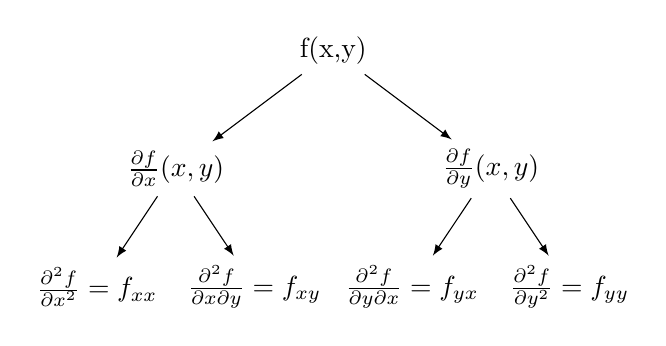
\begin{tikzpicture}[
        level 1/.style={sibling distance=40mm},
        level 2/.style={sibling distance=20mm},
        edge from parent/.style={draw, -latex}
    ]
    \node {f(x,y)}
        child {node {$\frac{\partial f}{\partial x} (x,y)$}
            child {node {$\frac{\partial^2 f}{\partial x^2} = f_{xx}$}}
            child {node {$\frac{\partial^2 f}{\partial x \partial y} = f_{xy}$}}
        }
        child {node {$\frac{\partial f}{\partial y} (x,y)$}
            child {node {$\frac{\partial^2 f}{\partial y \partial x} = f_{yx}$}}
            child {node {$\frac{\partial^2 f}{\partial y^2} = f_{yy}$}}
        };
    \end{tikzpicture}
\end{center}

\[
\nabla f = \begin{pmatrix}
    \dfrac{\partial f}{\partial x} &
    \dfrac{\partial f}{\partial y}
\end{pmatrix}
\]

\subsection*{Hessian Matrix}
\[
H = \begin{pmatrix}
    f_{xx} & f_{xy} \\
    f_{yx} & f_{yy}
\end{pmatrix}
\]

\subsection{Partial Differential Equations (PDEs)}
\subsection*{Problem 2}
\[
u(x,y,z) = \frac{1}{\sqrt{x^2 + y^2 + z^2}}, \quad (x,y,z) \neq (0,0,0)
\]
Where $u$ satisfies the PDE:
\[
u_{xx} + u_{yy} + u_{zz} = 0, \quad \text{which is } \Delta u = 0, \quad \textbf{Laplace's equation}
\]

\[
u = (x^2 + y^2 + z^2)^{-\frac{1}{2}}
\]
\[
u_x = -\frac{1}{2} \cdot (x^2 + y^2 + z^2)^{-\frac{3}{2}} \cdot 2x 
\]
\[
u_{xx} = \frac{3}{4} \cdot (x^2 + y^2 + z^2)^{-\frac{5}{2}} \cdot 2x^2 - \frac{1}{2} \cdot (x^2 + y^2 + z^2)^{-\frac{3}{2}}
\]
\[
u_{yy} = \frac{3}{4} \cdot (x^2 + y^2 + z^2)^{-\frac{5}{2}} \cdot 2y^2 - \frac{1}{2} \cdot (x^2 + y^2 + z^2)^{-\frac{3}{2}}
\]
\[
u_{zz} = \frac{3}{4} \cdot (x^2 + y^2 + z^2)^{-\frac{5}{2}} \cdot 2z^2 - \frac{1}{2} \cdot (x^2 + y^2 + z^2)^{-\frac{3}{2}}
\]

\[
u_{xx} + u_{yy} + u_{zz} = \frac{6}{4} \left(3(x^2 + y^2 + z^2)^{-5} - (x^2 + y^2 + z^2)^{-\frac{3}{2}} \right) = 0
\]

\subsection*{Problem 1}
\[
u_t = \alpha^2 u_{xx}, \quad \text{where } \alpha^2 \text{ is known as the diffusion coefficient in the } \textbf{heat equation}
\]

\[
u(x,t) = e^{-\alpha k^2 t} \cdot \sin(kx)
\]
\[
u_t = -\alpha k^2 e^{-\alpha k^2 t} \cdot \sin(kx)  
\]
\[
u_{x} = e^{-\alpha k^2 t} \cdot k \cdot \cos(kx)
\]
\[
u_{xx} = -e^{-\alpha k^2 t} \cdot k^2 \cdot \sin(kx)
\]

\subsection*{Problem 4c}
\[
u(x,t) = (x - at)^6 + (x + at)^6
\]
\[
u_{tt} = a^2 u_{xx} \quad \text{is known as the } \textbf{Wave equation}
\]

\subsection{Cross Derivatives}
\[
\text{When it is true that } \frac{\partial^2 f}{\partial x \partial y} = \frac{\partial^2 f}{\partial y \partial x}
\]

\paragraph{Theorem:} \textbf{Equality of Crossed Partial Derivatives} \\
Let $f : U \subset \mathbb{R}^n \rightarrow \mathbb{R}$ be defined on an open set $U$ and such that the partial derivatives $\frac{\partial f}{\partial x_i}$ and $\frac{\partial f}{\partial x_j}$ exist and are differentiable at $a \in U$. Then, $\forall x_i, x_j \in U$, it is true that:
\[
\frac{\partial^2 f}{\partial x_i \partial x_j} = \frac{\partial^2 f}{\partial x_j \partial x_i}, \quad \text{at } a
\]

\paragraph{Example}
\[ f(x,y) = 
\begin{cases}
    xy \cdot \dfrac{x^2 - y^2}{x^2 + y^2} & (x,y) \neq (0,0) \\
    0 & (x,y) = (0,0)
\end{cases}
\]

\[
\frac{\partial}{\partial x} \left(\frac{\partial}{\partial y} f\right) \big|_{(0,0)} \neq \frac{\partial}{\partial y} \left(\frac{\partial}{\partial x} f\right) \big|_{(0,0)}
\]

\[
\frac{\partial f}{\partial x} = 
\begin{cases}
    \dfrac{4x^2y^3 + x^4y - y^5}{(x^2 + y^2)^2} & (x,y) \neq (0,0) \\
    \lim_{t \to 0} \dfrac{f(t,0) - f(0,0)}{t} = 0 & (x,y) = (0,0)
\end{cases}
\]

\[
\frac{\partial f}{\partial y} =
\begin{cases}
    \dfrac{x^5 - 4x^3y^2 - xy^4}{(x^2 + y^2)^2} & (x,y) \neq (0,0) \\
    \lim_{t \to 0} \dfrac{f(0,t) - f(0,0)}{t} = 0 & (x,y) = (0,0)
\end{cases}
\]

\[
\frac{\partial^2 f}{\partial x \partial y} \big|_{(0,0)} = \lim_{t \to 0} \dfrac{\dfrac{\partial f}{\partial x}(0,t) - \dfrac{\partial f}{\partial x}(0,0)}{t} = \lim_{t \to 0} \dfrac{\dfrac{h^5}{h^4} - 0}{h} = 1   
\]

\[
\frac{\partial^2 f}{\partial y \partial x} \big|_{(0,0)} = \lim_{t \to 0} \dfrac{\dfrac{\partial f}{\partial y}(0,t) - \dfrac{\partial f}{\partial y}(0,0)}{t} = \lim_{t \to 0} \dfrac{-\dfrac{h^5}{h^4} - 0}{h} = -1   
\]

\subsection{Theorem}
Let $f : U \subset \mathbb{R}^n \rightarrow \mathbb{R}$ be defined on an open set $U$ and such that all the partial derivatives exist and are continuous at $a \in U$. Then, $f$ is differentiable at $a$ and its differential is given by the Jacobian matrix $Jf \big|_a$.

\paragraph{Proof}
\[
\lim_{h \to 0} \frac{f(a + h) - f(a) - Jf \big|_a \cdot h}{\| h \|} = 0
\]

\[
a = \begin{pmatrix}
    a_1 \\
    a_2 \\
    \vdots \\
    a_n
\end{pmatrix}, \quad h = \begin{pmatrix}
    h_1 \\
    h_2 \\
    \vdots \\
    h_n
\end{pmatrix}
\]

\[
a + h = \begin{pmatrix}
    a_1 + h_1 \\
    a_2 + h_2 \\
    \vdots \\
    a_n + h_n
\end{pmatrix} - \begin{pmatrix}
    a_1 \\
    a_2 + h_2\\
    \vdots \\
    a_n + h_n
\end{pmatrix} + \begin{pmatrix}
    a_1 \\
    a_2 + h_2 \\
    \vdots \\
    a_n + h_n
\end{pmatrix} + \ldots - \begin{pmatrix}
    a_1 \\
    a_2 \\
    \vdots \\
    a_n + h_n
\end{pmatrix} + \begin{pmatrix}
    a_1 \\
    a_2 \\
    \vdots \\
    a_n + h_n
\end{pmatrix}
\]

\[
f(a + h) = f\begin{pmatrix}
    a_1 + h_1 \\
    a_2 + h_2 \\
    \vdots \\
    a_n + h_n
\end{pmatrix} - f\begin{pmatrix}
    a_1 \\
    a_2 + h_2\\
    \vdots \\
    a_n + h_n
\end{pmatrix} + f\begin{pmatrix}
    a_1 \\
    a_2 + h_2 \\
    \vdots \\
    a_n + h_n
\end{pmatrix} + \ldots - f\begin{pmatrix}
    a_1 \\
    a_2 \\
    \vdots \\
    a_n + h_n
\end{pmatrix} + f\begin{pmatrix}
    a_1 \\
    a_2 \\
    \vdots \\
    a_n + h_n
\end{pmatrix}
\]

\[
f(a + h) - f(a) = f\begin{pmatrix}
    a_1 + h_1 \\
    a_2 + h_2 \\
    \vdots \\
    a_n + h_n
\end{pmatrix} - f\begin{pmatrix}
    a_1 \\
    a_2 + h_2\\
    \vdots \\
    a_n + h_n
\end{pmatrix} + f\begin{pmatrix}
    a_1 \\
    a_2 + h_2 \\
    \vdots \\
    a_n + h_n
\end{pmatrix} + \ldots - f\begin{pmatrix}
    a_1 \\
    a_2 \\
    \vdots \\
    a_n + h_n
\end{pmatrix} + f\begin{pmatrix}
    a_1 \\
    a_2 \\
    \vdots \\
    a_n + h_n
\end{pmatrix} - f\begin{pmatrix}
    a_1 \\
    a_2 \\
    \vdots \\
    a_n
\end{pmatrix}
\]

\[
f(a + h) - f(a) = D_{v_1} f \cdot h_1 + D_{v_2} f \cdot h_2 + \ldots + D_{v_n} f \cdot h_n
\]

\[
\text{Where } v_i = \begin{pmatrix}
    0 \\
    \vdots \\
    1 \\
    \vdots \\
    0
\end{pmatrix} \text{ is the } i \text{th unit vector}
\]

\[
f(a + h) - f(a) = \begin{pmatrix}
    \dfrac{\partial f_1}{\partial x_1} \\
    \vdots \\
    \dfrac{\partial f_m}{\partial x_1}
\end{pmatrix} \cdot h_1 + \begin{pmatrix}
    \dfrac{\partial f_1}{\partial x_2} \\
    \vdots \\
    \dfrac{\partial f_m}{\partial x_2}
\end{pmatrix} \cdot h_2 + \ldots + \begin{pmatrix}
    \dfrac{\partial f_1}{\partial x_n} \\
    \vdots \\
    \dfrac{\partial f_m}{\partial x_n}
\end{pmatrix} \cdot h_n
\]

So:
\[
\begin{pmatrix}
    \dfrac{\partial f_1}{\partial x_1} \big|_{x_1} & \dfrac{\partial f_1}{\partial x_2} \big|_{x_2} & \ldots & \dfrac{\partial f_1}{\partial x_n} \big|_{x_n} \\
    \dfrac{\partial f_2}{\partial x_1} \big|_{x_1} & \dfrac{\partial f_2}{\partial x_2} \big|_{x_2} & \ldots & \dfrac{\partial f_2}{\partial x_n} \big|_{x_n} \\
    \vdots & \vdots & \ddots & \vdots \\
    \dfrac{\partial f_m}{\partial x_1} \big|_{x_1} & \dfrac{\partial f_m}{\partial x_2} \big|_{x_2} & \ldots & \dfrac{\partial f_m}{\partial x_n} \big|_{x_n}
\end{pmatrix} \begin{pmatrix}
    h_1 \\
    h_2 \\
    \vdots \\
    h_n
\end{pmatrix}
\]

Finally:
\[
\lim_{h \to 0} \frac{f(a + h) - f(a) - Jf \big|_a \cdot h}{\| h \|} = \frac{Jf h - Jf \big|_a h}{\| h \|} = \frac{(Jf - Jf \big|_a) \cdot h}{\| h \|} = 0
\]
\[
Jf \big| \to Jf \big|_a \quad \text{as } h \to 0
\]

\end{document}